% Created 2019-05-02 Thu 14:37
% Intended LaTeX compiler: pdflatex
\documentclass[12pt, a4paper]{thesis}
\usepackage[utf8]{inputenc}
\usepackage[T1]{fontenc}
\usepackage{graphicx}
\usepackage{grffile}
\usepackage{longtable}
\usepackage{wrapfig}
\usepackage{rotating}
\usepackage[normalem]{ulem}
\usepackage{amsmath}
\usepackage{textcomp}
\usepackage{amssymb}
\usepackage{capt-of}
\usepackage{hyperref}
\usepackage{latex_config}
\usepackage{makeidx}
\makeindex
\setcounter{secnumdepth}{4}
\author{Simon Schnake}
\date{\today}
\title{Energy Regression with Deep Learning in Particle Collider Physics}
\hypersetup{
  pdfauthor={Simon Schnake},
  pdftitle={Energy Regression with Deep Learning in Particle Collider Physics},
  pdfkeywords={},
  pdfsubject={},
  pdfcreator={Emacs 26.2 (Org mode 9.1.9)}, 
  pdflang={English}}
\begin{document}

\begin{titlepage}
  % Fehler "destination with the same identifier" unterdrücken...
  \setcounter{page}{-1}
  \BgThispage
  {\fontfamily{phv}\selectfont
    % Titelseite
    \begin{figure}[h]
      \begin{minipage}[b]{62mm}
        
\includegraphics[width=62mm]{../images/unilogo}
      \end{minipage}
      \hspace{4cm}
      \begin{minipage}[b]{59mm}
        
\includegraphics[width=59mm]{../images/minlogo}
      \end{minipage}
    \end{figure}

    \vfill


    \begin{center}
      \uppercase{
        \noindent { \huge
          Masterarbeit \\
        }
        \vspace{12mm}
        % Titel
        \noindent \rule{\textwidth}{0.6mm} \\
        \noindent \textbf{\huge
          Energy Regression with Deep Learning in Particle Collider Physics\\
        }
        \noindent \rule{\textwidth}{0.6mm} \\
        \vspace{55mm}	}
    \end{center}
    
    \vfill
    \large{
      \noindent \hspace{0.25cm}\vspace{-0.25cm}\textbf{Simon Schnake} \\
      \noindent \rule{\textwidth}{0.4mm} 
      \noindent{simon.schnake@desy.de} \\
      \noindent{Studiengang Physik} \\
      \noindent{Matr.-Nr. 6506821} \\
      \noindent{6. Fachsemester} \\
      \begin{tabbing}
	\hspace{8em} \=  \kill
	Erstgutachter: \> Prof. Dr. Peter Schleper \\
	Zweitgutachter: \> Prof. Dr. Gregor Kasieczka \\
	~ \\
	Abgabe: 05.2019
      \end{tabbing}}}
    
    % Rückseite der Titelseite mit Zitat
    \newpage 
    \thispagestyle{empty}
  \setcounter{page}{0}

  ~\\ \vfill \noindent
  Dort standen auch Grenzsteine,\\
  etwas Überflüssiges, wie ihm erschien.\\
  \textit{-- Hermann Lenz}
\end{titlepage}








\chapter*{Abstract}

One of the fundamental questions of machine learning in particle
physics is whether we can improve the resolution of our measuring
instruments. Is it possible to gain deeper insights from the
structure? This question is examined in this thesis using the example
of calorimeter data and jet analysis. Different types of networks will
be investigated. The technique of the loss function design was
examined, which allows to reduce systematics in the data
structure. Overall, it is shown that deep learning can achieve better
performance in the application cases.

\chapter*{Zusammenfassung}
Eine der grundlegenden Fragen des Machinellen Lernens in der
Teilchenphysik ist ob wir die Auflösung unser Messinstrumente
verbessern können. Ist es möglich aus der Struktur tiefere
Erkenntnisse zu gewinnen. Diese Fragestellungen werden in dieser
Arbeit am Beispiel von Calorimeter Daten und der Jet Analyse
betrachtet. Es werden unterschiedliche Netzwerktypen
ausgetestet. Hierbei wurden Technik des Loss Funktionsdesigns erprobt,
die es erlauben Systematiken in der Datenstruktur zu
vermindern. Insgesamt wird dargestellt, das mittels Deep Learning sich
eine bessere Performance in den Anwendungsfällen erzielen lässt.

\tableofcontents
\cleardoublepage

\chapter{Introduction}
\label{sec:org1373fac}

Particle collisions such as those at the Large Hadron Collider (LHC)
\cite{lhc_machine} produce gigantic amounts of data. With the High
Lumi Upgrade \cite{bruening19_high_lumin_large_hadron_collid}, this
amount will increase considerably, requiring new analysis
techniques to gain new insights from the data. The progress in the
area of machine learning in recent years offers a toolbox of new
analysis techniques that can be applied to particle physics. In this
thesis some possibilities of this application are presented.

This work does not remain the only one in this pursuit, in recent
years considerable progress has been made in certain areas of particle
physics using deep learning. One aspect is that existing searches can
be supported by the help of deep learning
\cite{baldi14_searc_exotic_partic_high_energ,baldi15_enhan_higgs_boson_to_with_deep_learn,santos17_machin_learn_techn_searc_decay_chann}.
Furthermore it is also possible to use deep learning for model
independent searches
\cite{dagnolo19_learn_new_physic_from_machin,simone19_guidin_new_physic_searc_with_unsup_learn,heimel19_qcd_or_what}.
Pile-up can be detected
\cite{komiske17_pileup_mitig_with_machin_learn_pumml}.  In addition,
machine learning can be used to identify jets
\cite{komiske19_energ_flow_networ,cogan15_jet_images,oliveira16_jet_images_deep_learn_edition,baldi16_jet_subst_class_high_energ,barnard17_parton_shower_uncer_jet_subst,kasieczka17_deep_learn_top_tagger_or_end_qcd,datta17_how_much_infor_is_jet,komiske17_deep_learn_color}.
These are merely a few examples from the broad field of research that
was established in recent years.

This work will deal with low level data, especially calorimeter cell
data, and with high level variables such as clustered particles from
individual jets.  The aim here is to apply different techniques in
order to improve the energy resolution of those devices.

The following chapter gives a brief overview of particle physics. The
third chapter is following up with a discussion over particles
introducing matter and of calorimetry. Afterwards, Geant5, one of the
most commonly used analysis tools, is presented. In chapter 5 the
Large Hadron Collider, the CMS Detector, the Particle Flow Algorithm
as well as jet clustering and energy correction are described. Some
aspects of deep learning that play an important role in this work are
discussed afterwards. In the seventh chapter the first part of the
analysis will be presented. This part presents the application of some
deep learning algorithms in calorimetry resolution improvement. In the
second part of the analysis, the developed techniques and a special
form of a neural net, the `Particle Flow Network` are applied to jet
calibration. Chapter 9 concludes the work with a summary and an
outlook.

\chapter{Particle Physics}
\label{sec:orgcd2d7c7}
This chapter briefly outlines the core areas of particle
physics. Which are relevant for this work. The Standard Model of
Particle Physics and further topics are considered.

\section{The Standard Model of Particle Physics}
\label{sec:org862e92f}
The Standard Model of Elementary Particle Physics summarizes the
theoretical foundations of modern particle physics and describes the
elementary particles and the fundamental interactions of physics. It
contains a quantum field theoretical formulation of the
electromagnetic, the weak and the strong interaction as well as the
Higgs mechanism. The comparatively weak gravitation is not included.

\section{Fundamental Building Blocks}
\label{sec:org4008fdf}
The fundamental building blocks of matter are the elementary particles assumed
to be point-like. Elementary particles can be divided into bosons and fermions
according to their intrinsic angular momentum, the spin. Bosons have
an integer positive spin and fermions have a positive half spin.

\begin{figure}[H]

  \begin{tikzpicture}[x=1.2cm, y=1.2cm]
    \draw[round] (-0.5,0.5) rectangle (4.4,-1.5);
    \draw[round] (-0.6,0.6) rectangle (5.0,-2.5);
    \draw[round] (-0.7,0.7) rectangle (5.6,-3.5);

    \node at(0, 0)   {\particle[gray!20!white]
      {$u$}        {up}       {$2.3$ MeV}{1/2}{$2/3$}{R/G/B}};
    \node at(0,-1)   {\particle[gray!20!white]
      {$d$}        {down}    {$4.8$ MeV}{1/2}{$-1/3$}{R/G/B}};
    \node at(0,-2)   {\particle[gray!20!white]
      {$e$}        {electron}       {$511$ keV}{1/2}{$-1$}{}};
    \node at(0,-3)   {\particle[gray!20!white]
      {$\nu_e$}    {$e$ neutrino}         {$<2$ eV}{1/2}{}{}};
    \node at(1, 0)   {\particle
      {$c$}        {charm}   {$1.28$ GeV}{1/2}{$2/3$}{R/G/B}};
    \node at(1,-1)   {\particle 
      {$s$}        {strange}  {$95$ MeV}{1/2}{$-1/3$}{R/G/B}};
    \node at(1,-2)   {\particle
      {$\mu$}      {muon}         {$105.7$ MeV}{1/2}{$-1$}{}};
    \node at(1,-3)   {\particle
      {$\nu_\mu$}  {$\mu$ neutrino}    {$<190$ keV}{1/2}{}{}};
    \node at(2, 0)   {\particle
      {$t$}        {top}    {$173.2$ GeV}{1/2}{$2/3$}{R/G/B}};
    \node at(2,-1)   {\particle
      {$b$}        {bottom}  {$4.7$ GeV}{1/2}{$-1/3$}{R/G/B}};
    \node at(2,-2)   {\particle
      {$\tau$}     {tau}          {$1.777$ GeV}{1/2}{$-1$}{}};
    \node at(2,-3)   {\particle
      {$\nu_\tau$} {$\tau$ neutrino}  {$<18.2$ MeV}{1/2}{}{}};
    \node at(3,-3)   {\particle[orange!20!white]
      {$W^{\hspace{-.3ex}\scalebox{.5}{$\pm$}}$}
      {}              {$80.4$ GeV}{1}{$\pm1$}{}};
    \node at(4,-3)   {\particle[orange!20!white]
      {$Z$}        {}                    {$91.2$ GeV}{1}{}{}};
    \node at(3.5,-2) {\particle[green!50!black!20]
      {$\gamma$}   {photon}                        {}{1}{}{}};
    \node at(3.5,-1) {\particle[purple!20!white]
      {$g$}        {gluon}                    {}{1}{}{color}};
    \node at(5,0)    {\particle[gray!50!white]
      {$H$}        {Higgs}              {$125.1$ GeV}{0}{}{}};
    \node at(6.1,-3) {\particle
      {}           {graviton}                       {}{}{}{}};

    \node at(4.25,-0.5) [force]      {strong nuclear force (color)};
    \node at(4.85,-1.5) [force]    {electromagnetic force (charge)};
    \node at(5.45,-2.4) [force] {weak nuclear force (weak isospin)};
    \node at(6.75,-2.5) [force]        {gravitational force (mass)};

    \draw [<-] (2.5,0.3)   -- (2.7,0.3)          node [legend] {charge};
    \draw [<-] (2.5,0.15)  -- (2.7,0.15)         node [legend] {colors};
    \draw [<-] (2.05,0.25) -- (2.3,0) -- (2.7,0) node [legend]   {mass};
    \draw [<-] (2.5,-0.3)  -- (2.7,-0.3)         node [legend]   {spin};

    \draw [mbrace] (-0.8,0.5)  -- (-0.8,-1.5)
    node[leftlabel] {6 quarks\\(+6 anti-quarks)};
    \draw [mbrace] (-0.8,-1.5) -- (-0.8,-3.5)
    node[leftlabel] {6 leptons\\(+6 anti-leptons)};
    \draw [mbrace] (-0.5,-3.6) -- (2.5,-3.6)
    node[bottomlabel]
    {12 fermions\\(+12 anti-fermions)\\increasing mass $\to$};
    \draw [mbrace] (2.5,-3.6) -- (5.5,-3.6)
    node[bottomlabel] {5 bosons\\(+1 opposite charge $W$)};

    \draw [brace] (-0.5,.8) -- (0.5,.8) node[toplabel]         {standard matter};
    \draw [brace] (0.5,.8)  -- (2.5,.8) node[toplabel]         {unstable matter};
    \draw [brace] (2.5,.8)  -- (4.5,.8) node[toplabel]          {force carriers};
    \draw [brace] (4.5,.8)  -- (5.5,.8) node[toplabel]       {Goldstone\\bosons};
    \draw [brace] (5.5,.8)  -- (7,.8)   node[toplabel] {outside\\standard model};

    \node at (0,1.2)   [generation] {1\tiny st};
    \node at (1,1.2)   [generation] {2\tiny nd};
    \node at (2,1.2)   [generation] {3\tiny rd};
    \node at (2.8,1.2) [generation] {\tiny generation};
  \end{tikzpicture}
  \caption{A diagram of the standard model of particle physics. A comprehensive overview of the current understanding of the universe}
  \label{standarmodel}
\end{figure}

There exists twelve fermions in the framework of the Standard
Model. Fermions are particles with spin \(s = 1/2\). These fermions
form the fundamental components of matter. They are presented in
\ref{standarmodel}. They are categorized into three different
generations of fermions and quarks. A lepton generation consists of a
particle with a charge of \(-e\) and a corresponding neutralino. The
quark generations each contain a positive quark with charge \(2/3 e\)
and a negative quark with charge \(- 1/3 e\). The individual
generations are sorted according to their masses. Besides the charge
and the spin, the fermions have other quantum numbers, the weak
isospin and the quarks have an additional color charge. The color
charge is subdivided into red, green and blue. Each color represents
the coupling of the quarks to the strong interaction. Similarly, the
coupling to the weak interaction is associated with the weak
isospin. The weak isospin is correlated to the characteristic of
chirality which characterizes the handiness of a fermion corresponding
to a left-handed and right-handed projection. Corresponding to the
introduced quantum numbers, each of the twelve fermions has a
corresponding antiparticle, which results from the conjunction of
charge and parity and time.

\section{Fundamental Interactions}
\label{sec:org8c44b2a}

Electromagnetic, weak and strong interactions described by the SM can be
represented mathematically by an \(U(1)_{Y}, SU(2)_{T}\) and \(SU(3)_{C}\)
symmetry. These are called gauge groups or gauge symmetries. The gauge bosons
resulting from the linear combination of the respective generators of the gauge
groups are the photon, the W- and Z-boson and eight gluons. The photon
represents the alternating particle of the electromagnetic interaction and
couples to the electric charge q. Electromagnetism is described by quantum
electrodynamics (QED).

The W- and Z-boson are the interaction particles of the weak interaction and
couple to the weak isospin. Within the framework of the weak interaction,
coupling to the W-boson allows a transition between quark generations and also
lepton generations. The weak and electromagnetic interaction can be combined via
\(U(1)_{Y} \otimes SU(2)_{T}\) to the electroweak interaction. The gluons couple
to the color charge C and represent the interaction particles of the strong
interaction. The explicit couplings and processes are described in quantum
chromodynamics (QCD).  It follows from the formulation of the interactions by
gauge groups that gauge bosons must represent massless particles in order to
guarantee the required local gauge invariance of the Lagrangian density of the
SM. 

\section{Jets}
\label{sec:org85fb1e4}

The high-energy phenomena of quantum chromodynamics are described by
the color-charged particles, the quarks and the gluons. These
particles cannot be observed in isolation. Rather, the process of
hadronization causes directional bundles of color-neutral hadrons,
known as jets, to form. In the case of the LHC, protons are brought
into collision, but strictly speaking, the individual partons from the
protons collide with each other. Depending on the momentum of the
protons, the probability of their individual partons interacting
varies. To some extent, the effects involved can be described by the
probability density of the partons. The parton distribution density
indicates the probability of finding a parton of type i with a certain
longitudinal distance \(x\) in a hadron. Using the proton as an
example, it becomes clear that it is more likely to find quarks for
higher distances \(x\). In contrast, the gluons predominate within
small distance.

\begin{figure}[H]
  \centering
  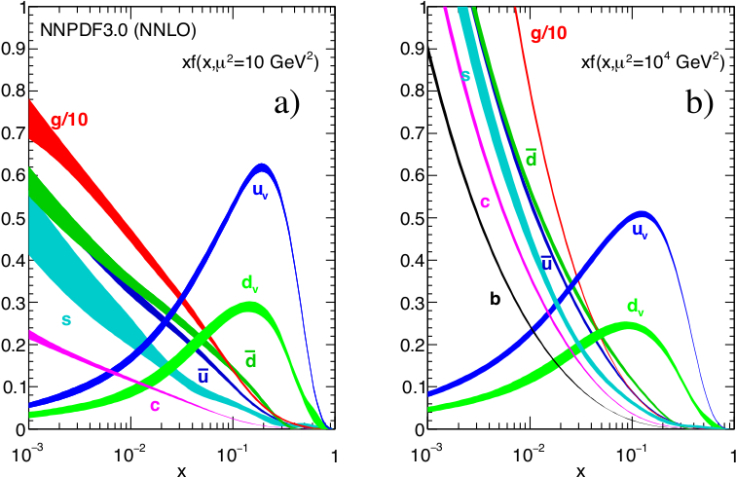
\includegraphics[width=0.8 \textwidth]{../images/partondensity.jpeg}
  \caption{Representation of the distribution of the momentum fraction x of a parton multiplied by its parton distribution function f(x). The two graphs show the distribution at different energy transfers \cite{PhysRevD.98.030001}.}
  \label{bremsstrahlung}
\end{figure}



The new parton created during the collision will typically radiate
further partons, resulting in a so-called parton shower. Partons bind
together during the hadronization process to form hadrons which are
observable. Many hadrons have a short lifetime and decay after a short
period of time. For this reason, a jet in the detector consists of
relatively few particle types, which together allow conclusions to be
drawn about the original parton.

\chapter{Calorimetry}
\label{sec:org802b29d}

This chapter discusses the fundamental interactions between particles and
matter.  Building on this, the principles of
electromagnetic and hadronic calorimeters are explained.

\section{Energy Loss Due to Ionisation}
\label{sec:org57bbfcf}

Charged particles moving through a medium lose energy through
individual, stochastically occurring collisions with the atoms of the
material. The collisions cause ionization, excitation of the atom, or
collective excitation of the medium.  The energy loss due to a
collision is usually low. In rare cases, a larger part of the energy
loss will be converted to the energy of the particle.

The Bethe formula indicates the average energy loss of heavy charged particles

\begin{align}
  -\expval{\dv{E}{x}} = K z^2 \frac{Z}{A} \frac{1}{\beta^{2}} \left[ \frac{1}{2} \ln{\frac{2 m_{e} c^{2} \beta^{2} \gamma^{2} T_{\text{max}}}{I^{2}}}-\beta^{2} - \frac{\delta(\beta\gamma)}{2}\right].
\end{align}

For small particle energies, the \(1/\beta^2\) term in the Bethe formula
dominates. As a result, particles that deposit their energy only
through ionization processes in the material, have a fixed range and
their energy deposition is greatest when this range is reached. The
characteristic peak in the energy deposition distribution is called
the Bragg peak.

\section{Interactions of Electrons}
\label{sec:org978e80c}

When passing through a material, electrons can deposit their energy in
two different ways \cite{kolanoski16}. On the one hand electrons
deposit their energy through the ionization of the medium, on the
other hand electrons lose their energy through the generation of
bremsstrahlung.  The energy loss of electrons through ionization
differs slightly from the ionization loss of heavy charged
particles. The reasons for this deviation are the kinematics, the
spin, the charge and the fact that the scattering observed in
ionization are the scattering of two identical particles
\cite{PhysRevD.98.030001}.  Bremsstrahlung is the loss of energy of
charged particles in the Coulomb field of an atomic nucleus by the
radiation of a photon. The bremsstrahlung thus runs analogously to a
Rutherford scattering under radiation of a photon.  The mean energy
loss due to bremsstrahlung can be approximately expressed by

\begin{align}
  \left( \dv{E}{x} \right) \simeq - \frac{E}{X_0}.
\end{align}

Since the energy losses due to ionization grow logarithmically with
the energy, while the bremsstrahlung losses increase linearly with the
energy \cite{PhysRevD.98.030001}, the dominant factor for high
energies is bremsstrahlung. With decreasing electron energy, the
losses due to ionization increasingly dominate. This is shown in
Figure \ref{bremsstrahlung}.

\begin{figure}[H]
  \centering
  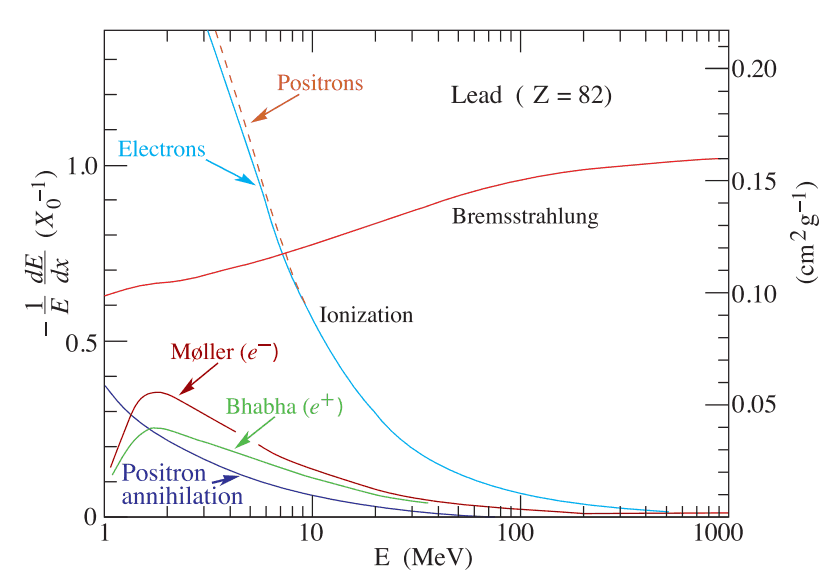
\includegraphics[width=0.8 \textwidth]{../images/bremsstrahlung.png}
  \caption{ Illustration of the different fractions of energy loss of
    electrons and positrons when passing through lead
    \cite{PhysRevD.98.030001}.}
  \label{bremsstrahlung}
\end{figure}

\section{Hadronic Interactions with Matter}
\label{sec:org39e1a53}

The development of hadronic showers is much more complicated than
electromagnetic showers \cite{wigman18}, which is due to the fact that
only a few processes play a role in electromagnetic showers.  Due to
the more diverse strong interaction, more diverse processes occur in
the development of hadronic showers. Another aspect that contributes
to the complexity of hadronic showers is that a struck nucleus
experiences nuclear interactions. In electromagnetic showers, whereas
the target only serves to scatter the particles involved in the shower
\cite{wigman18}.

Charged hadrons deposit part of their energy via the ionization of the
medium. Until they produce high-energy secondary particles in an absorption
process.  In contrast, neutral hadrons deposit their energy only by absorption
\cite{wigman18,fabjan03}. The mean free path between two hadronic interactions is
given by the hadronic absorption length \cite{fabjan03}. The hadrons produced in
the absorption process propagate further through the detector until they are
absorbed themselves.

The production of secondary hadrons in the nucleus takes place via the
process of spallation. The spallation is divided into two phases
\cite{wigman18}, the intranuclear cascade and evaporation.  At the
intranuclear cascade the incident hadron scatters on quasi-free
nucleons in the nucleus. These nucleons propagate further through the
nucleus and scatter to other nucleons. This forms a cascade of
particles in the core. During the formation of the intranuclear
cascade, pions and other unstable hadrons are formed. Some of the
particles generated escape from the nucleus and propagate further
through the medium. Thus contribute to the development of the hadronic
shower. The energies of the particles, which propagate further through
the medium are in the GeV range \cite{fabjan03}. Particles that do not
escape from the nucleus lead to a stimulus of the core. By emitting
free nucleons, $\alpha$ particles or heavier particles, the nucleus loses
this excitation energy again. The energy left in the core is radiated
via photons. The energy radiated from the nucleus in these two
processes is in the order of magnitude of some MeV \cite{fabjan03}.

The particles that lead to the development of the hadronic cascade are
protons, neutrons, and charged and neutral mesons
\cite{fabjan03}. Most of them are pions. One third of all pions
produced are neutral pions that electromagnetically decay into two
photons. This decay occurs before the neutral pions can interact
hadronically and results in a fraction of the energy of the hadronic
shower being converted into an electromagnetic sub-shower
\cite{fabjan03}. As the transmitted energy portion is no longer
available for hadronic interactions, the proportion of the
electromagnetic sub-shower increases with the energy of the of
incoming hadrons.

The electromagnetic part of a single shower fluctuates strongly, since
the electromagnetic fraction depends on the processes that take place
at the beginning of the shower \cite{wigman18}. In contrast to
electromagnetic showers the energy of a hadronic showers is not
completely detectable \cite{wigman18}. The reason is, that delayed
photons, soft neutrons, and the binding energy of hadrons and nucleons
are invisible to energy measurement \cite{fabjan03}. Due to differences
in the cross sections of the electromagnetic and the strong
interaction, hadronic showers have a significantly larger spatial
expansion than electromagnetic showers\cite{wigman18}.

\section{Calorimeter}
\label{sec:org937122c}

Calorimeters are used for destructive energy measurement by showers of incident
particles. Depending on the type of particle measured, they are subdivided into
electromagnetic and hadronic calorimeters. Calorimeters are divided into
homogeneous and sampling calorimeters. Homogeneous calorimeters are made of a
material that both acts as an absorber for the particles and simultaneously
generates the signal that can be measured. They consist of inorganic, heavy
scintillation crystals or non-scintillating Cherenkov radiators
\cite{PhysRevD.98.030001}. Sampling calorimeters consist of a sequence of active
and passive layers. In the passive layers the particles are absorbed and in the
active layers the signal is generated by ionization or scintillation. Materials
used in passive layers are typically lead, iron, copper and uranium. Liquid
noble gases, organic or inorganic scintillators are used in active layers
\cite{PhysRevD.98.030001}. The following two subsections deal with the properties
of electromagnetic and hadronic calorimeters.

\subsection{Electromagnetic Calorimeter}
\label{sec:em-calo}

The relative energy resolution of electromagnetic calorimeters is
given by 

\begin{align}
  \frac{\sigma}{E} = \frac{a}{\sqrt{E}} \otimes b \otimes \frac{c}{E}\ \cite{fabjan03,PhysRevD.98.030001}
\end{align}

The symbol \(\otimes\) stands for the square sum of the individual terms. The
first term is the stochastic term, the second the constant term and the third
the noise term.  The stochastic term is caused by fluctuations of the number of
charged tracks in the active medium. The stochastic term in sampling
calorimeters is proportional to

\begin{align}
  \frac{\sigma}{E}\propto \sqrt{\frac{t}{E}}.
\end{align}

Here \(t\) describes the thickness of the absorber in units of the
radiation length \(X_0\) and \(E\) is the energy of the incident
particle. In order to obtain this proportionality, it is necessary to
assume that the numbers of charged traces in the individual layers are
independently distributed and shaped in Gaussian form \cite{amaldi81}. The
noise term is caused by electrical noise in the signal processing and
the selection of the detector \cite{fabjan03}. The constant term is due to
energy-independent effects, such as inhomogeneities in the structure
of the detector, inaccuracies in fabrication, temperature gradients or
radiation damage \cite{fabjan03}.

\subsection{Hadronic Calorimeter}
\label{sec:orgd771604}

Since part of the energy deposited in a hadronic shower is not
detectable, a calorimeter generally provides a smaller signal for
hadrons than for electrons \cite{fabjan03}. A quantitative description
is given by the ratio e / h , which is therefore generally greater
than one \cite{wigman18}.

A calorimeter that delivers the same signals for a hadron and an
electron has a ratio of \(e / h = 1\) and is called a compensating
calorimeter \cite{wigman18}. Compensation is an internal property of a
calorimeter \cite{kolanoski16} and cannot be measured directly
\cite{wigman18}. The \(e / h\) ratio is determined by measuring the
\(e / \pi\) ratio \cite{wigman18}. The \(e / \pi\) ratio indicates the
ratio of the signals of an electron and a pion and is defined by

\begin{align}
  \frac{e}{\pi}=\frac{e/h}{1-f_{\text{em}} - e/h}. \cite{wigman18}
\end{align}

Therefore, the \(e / \pi\) ratio of the electromagnetic shower fraction
\(f_{\text{em}}\) depends on the energy of the incident pion. The \(e / \pi\) ratio
is independent to large energies from the compensation of the calorimeter and
strives towards one.

Compensation improves the linearity and resolution of a hadronic calorimeter
\cite{wigman18,kolanoski16,fabjan03}, The response of non-compensating
calorimeters is not linear, since the electromagnetic part of the shower
increases with the increasing energy of the incident particle. Since the
electromagnetic component has a stronger signal, the response of a
non-compensating calorimeter to particles of higher energy is larger. The
resolution of the calorimeter also improves if compensation is present. The
proportion of the electromagnetic shower component fluctuates strongly. If a
calorimeter is not compensating, signals of different magnitudes are generated
from events by the same energy and the resolution deteriorates.

Compensation is therefore a design criterion for hadronic
calorimeters. In general, \(e / h > 1\) applies. Therefore, a
reduction of the electromagnetic signal while simultaneously
increasing the hadronic signal leads to compensation. Therefore, by
using absorber materials with with high numbers of nuclear charges,
the electromagnetic signal can be reduced. A large part of the energy
deposition of electromagnetic showers takes place by absorption of
low-energy photons in the absorber. During these processes, electrons are
released that cannot reach the active medium in absorbers with high
nuclear masses and can therefore no longer contribute to the
signal. The magnification of the hadronic fraction is achieved by the
improved detection of cold evaporation neutrons. The energy transfer
of neutrons is inverse proportional to the molar mass of the
material. Therefore neutrons cross the passive medium without losing
energy and transfer their energy in the active medium via elastic
scattering to protons. These protons have a short range and therefore
do not reach the passive medium. The increase of the signal emitted by
the nuclear component of the shower can thus be achieved by variation
of the layer thicknesses of active and passive medium against each
other or by enrichment of the active medium with hydrogen.

\chapter{Geant4}
\label{sec:orgc423253}

The basics of simulating a detector with \emph{Geant4}  \cite{geant_simul_toolk} are discussed in this
chapter. The first section deals with the structure and sequence of a Geant4
application. The following two sections deal with the operation of particle
tracking by the detector and the simulation mechanisms. The last section of the
chapter discusses with the definition of a detector geometry.


\section{The Structure of a Simulation}
\label{sec:org08164e5}

Each Geant4 application passes through different states during a
simulation. These are the \texttt{preInit} state; a state during
initialization, a state from which a run is started, in which the
application is during the run, and a state that is passed through
while leaving the application. The first step in the simulation
process is to create an instance of the \texttt{RunManager} class that
controls the entire process \cite{geant4-doc} . Creating the
\texttt{RunManager} instance sets Geant4 to \texttt{preInit}
state. The classes, which are used to describe the components, are
transferred to the \texttt{RunManager} from this state
\cite{geant4-doc} . There are three required and five optional
classes. The required classes are the
\texttt{G4VUserDetector Construction} class, a physics list, and a
\texttt{G4PrimaryGeneratorAction} class, which is used to generate
primary particles and vertices. The used detector geometry is defined
by the \texttt{G4VUserDetectorConstruction} class. The
\texttt{G4PrimaryGeneratorAction} class is used to generate the
initial state of the simulation. The initial state can be made
available by the interface to a framework \cite{geant_simul_toolk}
. On the other hand, the \texttt{G4ParticleGun} class provides the
possibility to generate primary particles and vertices. It allows the
selection of a primary particle and the setting of dynamic properties
such as momentum, kinetic energy, location and flight
direction. Furthermore, there is the option to generate several
particles at once or to assign a polarization direction to the
particle \cite{geant4-doc}. After the submission of the classes to the
\texttt{RunManager} the initialization of the kernel takes place. It
starts with calling the \texttt{Initialize} method of the
\texttt{RunManager}. During the initialization the application is in
the initialization state and changes to the standby state after
successful execution \cite{geant4-doc}. From this state the start of a
simulation run takes place by calling the \texttt{BeamOn} method of
the \texttt{RunManager} class. As argument it expects the number of
events to be simulated.  The simulation is divided into different
simulation units, which are hierarchically structured. The individual
units represent smaller and smaller building blocks of the simulation.
The largest simulation unit is a run. A run consists of several events
and is started by calling the \texttt{BeamOn} method
\cite{geant4-doc,geant4-rec-dev}. An event consists of the decay or
interaction of the primary particle or particles
\cite{geant4-rec-dev}. At the beginning of the simulation the event
contains information about the primary particle and the primary
vertex. These are converted during the simulation, and after the
simulation, the event contains information about the trajectories of
the particles by the detector as well as about hits registered in the
detector \cite{geant_simul_toolk}. The next smaller simulation unit is
a track. A track represents a particle moving through the detector
\cite{geant4-doc}. It consists of several steps. A track contains
static information about the transported particle, such as the charge
or mass of the particle, as well as dynamic properties that change
during simulation. Dynamic properties include momentum, kinetic
energy, and the location of the particle. The trace of the particle
exists until the particle comes to rest or decays \cite{geant4-doc}. A
step contains information about the beginning and the end point
\cite{geant4-doc}. The length of a step is limited by the distance to
the next volume, the energy loss by continuous processes or by its
limitation in the \texttt{G4UserLimit} class \cite{geant_simul_toolk}.
The kernel can be initialized with five additional classes, which
enable the detector to interfere with the tracking of the particle at
the transition between the simulation units. There is a class for
manipulating each simulation unit, as well as a class with which the
priority of tracking a particular track by the detector can be
changed. This is the \texttt{G4UserStackingAction} class. The two
classes \texttt{G4UserRunAction} and \texttt{G4UserEventAction} can be
used to intervene in the simulation at the beginning and end of a run
or event. These classes are usually used for the analysis of a run or
event \cite{geant4-doc}. The class \texttt{G4UserTrackingAction} is
used to manipulate the tracking of the particle at the beginning and
end of a track. The \texttt{G4UserSteppingAction} class handles the
sequence of a step.

\section{Integration Of Physical Interactions}
\label{sec:org40783eb}

The integration of physical interactions into a simulation is done via
the physics list. The physics list determines the particles that occur
in the simulation and which interactions they experience. It can be
completely defined by the user. In addition, it is the possible to use
and extende a predefined reference physics list
\cite{geant4-rec-dev}. The definition of the physics list corresponds
to the assignment of all processes that a particle can experience
\cite{geant_simul_toolk}. The representation of physical interactions
is implemented by the Geant4 class \texttt{G4VProcess}
\cite{geant_simul_toolk}. The term process stands for the physical
interactions during the simulation and is managed by the class
\texttt{G4VProcess}. The interfaces of all processes are
identical. This enables a general handling of all processes by
tracking. The abstraction of the processes leads to a simple
possibility to add new processes to a simulation or to extend existing
processes in order to improve the accuracy of the simulation
\cite{geant4-doc}. Processes are divided into seven different
categories, which are electromagnetic, hadronic, optical, decay and
photoleptonic hadron processes. In addition, there is the category of
transport processes as well as the category of parameterization. A
further subdivision of the processes takes place according to the type
of interaction. A distinction is made between processes for particles
at rest that take place along the entire step and processes that occur
locally at the end of the step \cite{geant_simul_toolk}.

\section{Tracking}
\label{sec:org2ff4601}

The abstraction of physical interactions in processes with identical
interfaces makes it possible to describe the transport of any particle
through the detector with an algorithm. The tracking of a particle by
the detector can thus be carried out regardless of the observed
particles and physical interactions.  In Geant4, the transport of the
particles through the detector takes place step by step
\cite{geant_simul_toolk}.  At the beginning of a simulation step, each
process from the list of the observed particle suggests a step length
via its \texttt{GetPhysicalInteractionLength} method
\cite{geant_simul_toolk}. If the particle is at rest, only decay
processes are considered. In order to improve the accuracy of the
simulation, several mechanisms that additionally limit the step length
of a particle are used. On the one hand, processes that describe a
continuous energy loss suggest a step length. Furthermore, the
shortest distance of the present location to the next volume boundary
limits the step length.  This ensures that the particle does not pass
into any different volume during the step \cite{geant4-rec-dev}. The
smallest proposed step length determines the process being
performed. Processes associated with a loss of energy or a change of
direction of the particle can force their execution and take place
even if their proposed step length is not the shortest present
\cite{geant_simul_toolk}.

\section{Geometry}
\label{sec:org8d2fc6f}

The requirements for the definition of geometry are manifold. They range from
basic analyses of calorimeters up to complex detector assemblies at large-scale
experiments such as the Large Hadron Collider \cite{geant4_geom}. The definition
of the geometric objects that a detector contains is done in Geant4 in three
stages.  The first stage is the definition of a body. A Body is defined by its
shape and dimensions. The construction of the body is done by selecting the
appropriate shape from the available \texttt{Constructed Solid Geometries (CSG)}
\cite{geant4_geom}. The second level of the geometry definition is done by adding
physical properties to already predefined volumes. The resulting object is called
logical volume and is represented by the class \texttt{G4LogicalVolume}. The logical
volume contains the physical properties of the material it is made of. Further the
definition of the electromagnetic fields and the user-defined limitations belong
to a logical volume \cite{geant4-doc}. The third and last stage of the definition
of a detector is the positioning of the logical volumes in space. A placed
volume is called physical volume. In order to to describe the detector
completely, it is necessary for volumes to be inserted into each other.  The
world volume represents the largest volume in the definition of a detector. It
contains all other volumes, which describe the detector. The placed volumes are
called daughter volume and are surrounded by the mother volume.  The position of
the subsidiary volume is relatively to the center of the mother volume
\cite{geant4-doc}.

\section{Materials}
\label{sec:org11f3d27}

The structure of the materials in Geant4 replicates the structure of
materials in nature. Materials are composed of molecules or elements,
which in turn consist of isotopes \cite{geant_simul_toolk}. The
defining properties of an isotope are the name of the isotope, the
nuclear charge number, the nucleon number and the molar mass. An
element has the properties of name, nuclear charge, effective nucleon
number, effective molar mass and cross section per atom
\cite{geant4-doc}. An element is accessed via its symbol in the
periodic table of the elements.  An element is defined either by the
composition of the isotopes or directly by defining the effective
quantities. The effective cross section per atom is calculated from
the nuclear charge, the nucleon number and the molar mass
\cite{geant4-doc}. Analogous to the definition of an element from
isotopes, the definition of a material takes place.  Either a new
element with the effective values is generated or different elements
are combined to one material. A material is defined by its properties
such as density, state of aggregation, temperature and
pressure. Geant4 calculates the mean free path length, radiation
length, hadronic interaction length and the mean energy loss per
radiation length, which is given by the Bethe equation
\cite{geant4-doc}. The values of the physical quantities must be
defined in the program code. Furthermore, there is the possibility to
define materials from the internal database. This simplifies the
definition of materials, since all physical quantities of a material
can be isotops, elements or materials are provided.

\chapter{Experimental Setup}
\label{sec:org5cd8e52}
\section{The Large Hadron Collider}
\label{sec:orgf5b86e0}
The \emph{Large Hadron Collider} (LHC) \cite{lhc_machine} is the most powerful particle
accelerator in the world in terms of centre-of-mass energy and the frequency of
particle collisions. It is located at the European Organization for Nuclear
Research (Conseil européen pour la recherche nucléaire, CERN) near Geneva in
Switzerland. The storage ring was built in the tunnel of the former Large
Electron Positron Collider (LEP). The tunnel tube has a circumference of 26.7 km
and is located between 45m and 175m underground. The objectives of the LHC are
the investigation of physics beyond the standard model as well as precision
measurements. One of the greatest tasks and achievements of the LHC was the
discovery of the Higgs Boson in 2012 \cite{higgs_cms,higgs_atlas}. For this
purpose it was designed with a centre-of-mass energy of \(\sqrt{s} = 14\) TeV and
the associated luminosity of \(L = 10^{34} cm^{-2}s^{-1}\). 



\begin{figure}[H]
  \centering
  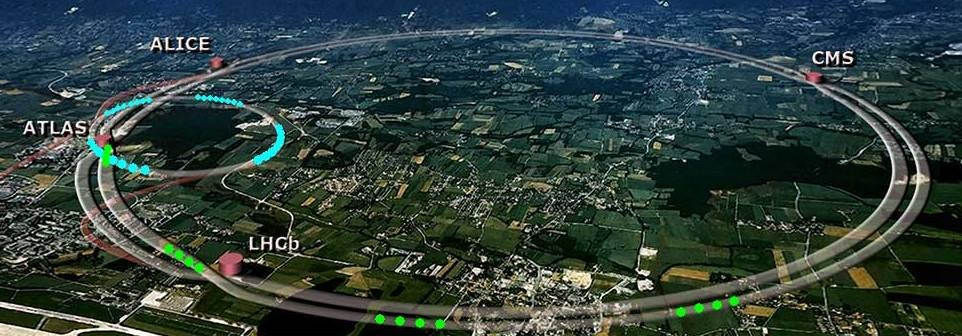
\includegraphics[width=\textwidth]{../images/lhc.jpeg}
  \caption{The graph shows the four main experiments (ALICE, ATLAS, CMS and LHCb) at the LHC \cite{lhcmap}}
  \label{4experiments}
\end{figure}



Luminosity describes the particle reactions per time and per area and is defined
as

\begin{align}
  \dv{N}{t} = L \sigma.
\end{align}

Here \(\dv{N}{t}\) is the number of reactions per time unit and
$\sigma$ is the cross section.  The luminosity is used especially for
the characterization of accelerators and provides information about
the expected particle rate. It can be calculated for a collision
experiment as

\begin{align}
  L = f \frac{N_{a}N_{b}}{4 \pi \sigma_{x} \sigma_{y}}
\end{align}

Here it is assumed that the radiation packets have a Gaussian density
profile with widths \(\sigma_{x,y}\) perpendicular to their flight
directions.  \(N_{a}\) and \(N_{b}\) represent the number of particles in
the two colliding particle bunches which repeatedly collide at the
frequency \(f\) in the experiment.  In the storage ring, protons are
accelerated in two adjacent vacuum tubes and collided in the centres
of four experiments. Figure \ref{4experiments} shows the LHC with its
four experiments: ALICE(A large Ion Collider Experiment) \cite{alice},
ATLAS(A Toroidal LHC ApparatuS) \cite{atlas}, CMS(Compact Muon
Solenoid) \cite{cms} and LHCb(LHC beauty) \cite{lhcb}.

\section{The CMS Experiment}
\label{sec:orge5edd5f}
The Compact Muon Solenoid Detector was specially developed to
characterize the proton-proton collisions at a center-of-mass energy
of 14 TeV. The CMS detector runs cylindrically around the beam axis
with a radius of 15m and a length of 21.6m. The basic setup including
the subcomponents of the CMS detector is shown in figure
\ref{cms-detector} in the transverse plane.  From the inside out, the
detector consists of a track detector, an electromagnetic calorimeter
(ECAL), a hadronic calorimeter (HCAL) and a muon system.  Inside the
muon system there is a superconducting solenoid magnet with a diameter
of about 6 m and a field strength of up to 4 T, which includes the
calorimeters and trace detectors.
\begin{figure}[H]
  \centering
  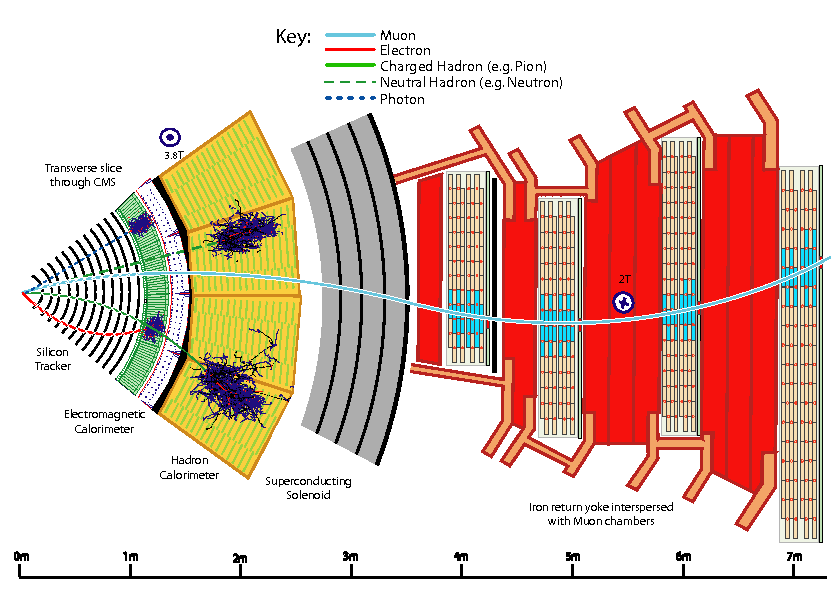
\includegraphics[width=0.8 \textwidth]{../images/cms_detector.png}
  \caption{Illustration of a tranverse slice of the CMS detector. Also specific particle interactions are shown \cite{sirunyan17}}
  \label{cms-detector}
\end{figure}

\subsection{Coordinate System and Conventions} %
\label{sec:org067f254}

For a precise description of the functionality and the construction of
the subcomponents, the coordinate system used in the CMS experiment is
introduced. In addition, further physical conventions are introduced.

The CMS experiment uses a right-handed Cartesian coordinate system which
originates at the collision point of both proton beams. Accordingly, the z-axis
points in the beam direction, the y-axis points upwards and the x-axis points in
the direction of the accelerator center. In addition to a Cartesian coordinate
system, polar coordinates are used for a simpler representation. Here the
azimuth half-angle \(\phi\) denotes the spanned angle in the x-y-plane and the polar
angle \(\theta\), starting from the z-axis, denotes the spanned angle in the
z-y-plane.
According to the use of both coordinate systems, the momentum in the transversal
plane of the detector, \(p_T\), is defined as

\begin{align}
  p_T = \sqrt{p_x^2 + p_y^2} = p \cdot \sin(\theta)
\end{align}

The invariance of the transverse pulse with respect to the Lorentz
transformation along the z-axis results in the angle size of the pseudorapidity
\(\eta\), which is also invariant under such transformations

\begin{align}
  \eta = - \ln(\tan(\theta/2))
\end{align}

Assuming a negligible mass compared to the energy of the physical objects under
consideration, an identity to rapidity is obtained 

\begin{align}
  y = \frac{1}{2} \ln(\frac{E+p_z}{E-p_z}).
\end{align}

On the basis of the pseudorapidity \(\eta\) and the azumuthal angle \(\phi\), a
formulation of the spatial angle distance \(\Delta R\), which is invariant with
respect to the Lorentz transformation along the z-axis, follows

\begin{align}
  \Delta R = \sqrt{(\Delta \eta)^{2} + (\Delta \phi)^{2}}.
\end{align}

In combination with the energy \(E\), \(\phi\), \(\eta\) and \(p_{T}\) describe all components of
the four-vector \(p_{\mu}\) of a particle. The invariant mass of the corresponding
particle is calculated from the four-vector

\begin{align}
  m^{2} = p^{\mu}p_{\mu}.
\end{align}

\subsection{Tracking Systems}
\label{sec:org139ed11}
The inner trace detector is dedicated to the identification of charged particles
and the reconstruction of associated trajectories. 

It consists of 1440 pixel and 15148 silicon strip detectors and covers a solid
angle range of up to \(\abs{\eta} = 2.5\). The individual pixel and strip
detectors each have an extension of \(150\mu \text{m} \times 100 \mu \text{m}\) or
\(80\mu \text{m} \times 10 \text{cm}\) and \(180\mu \text{m} \times 25 \text{cm}\).
This enables a spatial resolution of \(10\mu \text{m}\) for the pixel detectors
and \(23\mu \text{m}\) for the stripe detectors in the x-y plane and \(20\mu
\text{m}\) and \(230\mu \text{m}\) respectively along the beam axis.

\subsection{Electromagnetic Calorimeter}
\label{sec:orgf218141}

The electromagnetic calorimeter (ECAL) consists of 75848 homogeneous
PbWO4 crystals and has a solid angle granularity of
\(0.0174 \abs{\eta} \times 0.0174 \abs{\phi}\), providing a
homogeneous resolution. Furthermore, the ECAL covers a solid angle
range of up to \(\abs{\eta} = 3\). The lack of instrumentation from
\(1.479 < \abs{\eta} < 1.653\) is pointed out, subsequently this
region is unsuitable for the reconstruction of electrons and photons.
If the trajectory of an electron or photon is directed through ECAL,
such a particle emits energy in the form of emitted photons and
electrons from bremsstrahlung and pair production. The emitted photons
are measured by photodiodes with a relative energy resolution
\(\left( \frac{\sigma}{E} \right)^{2}\), where sigma is the resolution
of the measured energy

\begin{align}
  \left( \frac{\sigma}{E} \right)^{2} = \left( \frac{2.8}{\sqrt{E}} \right)^{2} + \left( \frac{0.12}{E} \right)^{2}+(0.3)^{2}.
\end{align}


\subsection{Hadron Calorimeter}
\label{sec:orgde6b415}
In contrast to ECAL, the hadronic calorimeter (HCAL) primarily detects
hadrons due to its higher material density. Hadrons interact via the
strong interaction with the detector material resulting in inelastic
reactions.  The energy deposited here is absorbed by
scintillators. Due to the high interaction length, the HCAL is more
extensive than the ECAL and therefore further away from the beam
axis. It is divided into a central region (HB), an outer central
region (HF), an end cap region (HE) and a forward region (HF) as shown
in Figure X. The HCAL is further divided into a central region (HB),
an outer central region (HF), an end cap region (HE) and a forward
region (HF). HB, HO and HE have a spatial angle granularity of
\(0.087[\eta] \times 0.087 [\phi]\), whereas the HF with
\(0.0175 [\eta] \times 0.0175 [\phi]\) has a much better angular
resolution.

Compared to the ECAL, the HCAL has a significantly inferior energy resolution

\begin{align}
  \left( \frac{\sigma}{E} \right) = \left( \frac{115.3}{\sqrt{E}} \right) + (5.5).
\end{align}

\subsection{Solenoid}
\label{sec:org004c39a}
The CMS detector has a superconducting solenoid magnet, which consists
of a cylindrical magnet coil with a diameter of 6 m and a length of
12.5 m.  The magnet is designed to generate a magnetic field of up to
4T inside the coil. The traces of charged particles are strongly
curved in the transversal plane, enabling the detector to measure
their momenta.

\subsection{The Muon System}
\label{sec:org643030a}

Most of the observed muons originate from the decay of heavier
particles and therefore indicate interesting physical processes. At
150.7 MeV they have a comparably low mass and hardly interact with the
calorimeters.  Therefore, nearly unscathed, the muons pass through the
inner detector components into the muon spectrometer, which is the
outermost detector layer. Most other particles decay or are absorbed
beforehand, so that almost every particle observed in this detector
system is a muon. The muon system serves both the identification and
the momentum measurement of muons and consists of several subsystems.
The muon spectrometer functions in interaction with the magnet. The
strong magnetic field it generates bends the particle path of the
muons in the transverse plane. The momentum of the muons is one of the
best measured quantities of the entire CMS detector, since the
particle is measured in the inner trace detector and in the muon
chamber. The blue curve in Figure \ref{cms-detector} shows a possible
trajectory of a muon which first is first bent in a 4 T magnetic field
in the inner trace detector and then deflected in the opposite
direction in a 2 T magnetic field. The muon spectrometer detects muons
in the range of \(\abs{\eta} < 2.4\). In addition, after all
transverse pulses of the directly detectable particles have been
determined in the last detector system, neutrinos can be indirectly
detected via the missing transverse momentum due to the conservation
of the entire transverse momentum.

\subsection{The Trigger System}
\label{sec:org9d9e9a7}
The proton bunches collide at the LHC at a rate of about 40 MHz, with
up to 100 proton pairs interacting simultaneously. Since the amounts
of data produced are too large for storage systems currently available
to be stored unfiltered, a preselection is made. This process is
carried by the trigger system. It should be noted that it is basically
not necessary to evaluate all events such as many of them are
so-called soft events. These events carry a small transverse impulse
and have been investigated in other experiments in the past. In this
case, it is sufficient only to record every Nth event. Likewise a
trigger system can select its events after the identification of
particle signatures. Thus, the information that the muons have been
identified in the muon system can be used as a trigger criterion. CMS
uses a two-stage trigger system. First the up to O(100 kHz) fast
Level-1 trigger from programmable hardware processors and then the
high-level trigger is used. The Level-1 trigger compares the recorded
data with the desired detection characteristics and forwards the data
to the high-level trigger if the characteristics are successfully
recognized. The higher level triggers performs a complete
reconstruction with the information from all detector components. The
reconstruction algorithm is similar to the algorithm used for later
data analysis. Only when events meet the requirements of this
selection level are they written to storage media for later data
analysis. Overall, the rate at which the CMS triggers is between 200
Hz and 1 kHz.

\section{Particle Flow}
\label{sec:org5293ff6}

The particle flow reconstruction algorithm is used in the CMS
experiment. The identification and reconstruction of individual
particles from the proton-proton collisions at the LHC is achieved by
combining the information from the different detector systems. By
combining the energy deposition in the calorimeters with the data
measured by the trace detector and the muon system, very small
uncertainties on the measured particle four-vectors are achieved. The
combination of the information is carried out with a view to an
optimal determination of the direction and energy of the
particles. Due to the different interactions in the detector, the
observed particle type can be determined with high probability.  The
CMS detector is ideally suited for the use of this algorithm as it has
a precise tracker. As shown in Figure \ref{cms-detector}, the muons
traverse all detector components and then leave signals in the inner
source detector and in the muon chambers. Photons deposit most of
their energy in the ECAL, whereas the charged leptons leave additional
traces in the trace detector. The pulse of the charged hadrons is
recorded in all positions up to HCAL, while neutral hadrons can only
be measured in the HCAL.

In the first step, the PF algorithm reconstructs the detected muons and elctrons
and subtracts them from the measured signals for further processing in order to
separate them from the possible candidates of the charged hadrons. The algorithm
merges the remaining traces with the energy depositions from the calorimeter. If
the measured energy in the calorimeter is compatible with the associated
reconstructed pulse of the trace, the associated signals are used to determine
the four-momentum of the hadron. However, if the energy deposited in ECAL or
HCAL is significantly higher than the corresponding values of the track, an
additional overlapping photon in ECAL or a neutral hadron in HCAL is
reconstructed along the track.

\section{Jet Clustering}
\label{sec:orgfca5f43}

A jet algorithm defines the rule for clustering individual particles into
jets. Jet algorithms usually have a resolution parameter that determines how
close two particles may be without being part of the same jet.

A large group of clustering algorithms can be defined by the general distance
metrics

\begin{align}
  d_{ij} = \min(p^{2k}_{T,i}, p^{2k}_{T,j}) \cdot \frac{\Delta^{2}_{ij}}{R^{2}} \label{jet_algo}
\end{align}


Here pt is the transverse momentum of a part l. delta describes the
distance between particles i and j in eta-phi space via

\begin{align}
  \Delta_{ij}^{2} = (\eta_{i} - \eta_{j})^{2} + (\phi_{i} - \phi_{j})^{2}
\end{align}

and R specifies the maximum radius if the shape of the jet is assumed
to be a cone in r-eta-phi space. The factor k determines the behavior
of the algorithm. For k=1 the equation \eqref{jet_algo} describes the
so-called k\_t algorithm, for k=-1 the anti k\_t algorithm and for k=0
the Cambridge/Aachen algorithm.

These algorithms fulfill two essential properties. They provide collinear and
infrared security. A jet algorithm is referred to as infrared safe if the
algorithm is stable against additional energetically weak radiation in the
jet. If the jet does not change its direction or its reconstructed energy when a
particle is split up in the jet, it is a jet algorithm with collinear
safety. CMS usually uses the anti-k\_t algorithm.

\section{Jet Energy Corrections}
\label{sec:org1fc0f38}

Due to detector defects, the energy of the reconstructed jets does not
match the true energy of the jets. The true energy is defined by the
energy of the original parton. Therefore, it is necessary to align the
energies of the jets with the true energies of the jets using jet
energy corrections. To assign the corrected energies to the
reconstructed jets, the differences between the reconstructed jets and
true jet energies are determined. In this way, detector-specific
effects, such as interactions in the material, are reduced.  The
jet corrections in CMS follow a fixed procedure.

The Level 1 (L1) correction reduces the shift of energy by
pile-up. The term pile-up describes the effects of events of
additional proton-proton interactions, whereby additional energy
deposition in the detector reconstructs a different energy than just
the energy of the jets from the interesting process. These corrections
are determined by comparing identical events from Monte Carlo
simulations with and without pile-up events. The resulting correction
factor depends on the transverse momentum of the jet pT, the
pseudorapidity of the jet eta, the jet area A and the mean density of
the transverse momentum rho, which are calculated using the kT
algorithm for R=0.6.

The L2L3 correction improves the energy of the reconstructed jets so
that it corresponds on average to the energy of the generated
jets. This is achieved by forming the ratio of the reconstructed
transverse momentum ptreco to the generated transverse momentum
ptgen. The ratio is referred to as the detector response

\begin{align}
  \mathcal{R} = \frac{p^{\text{reco}}_T}{p^{\text{gen}}_T}.
\end{align}


The moments \(p^{\text{reco}}_T\) and \(p^{\text{gen}}_T\) that belong
together are combined as responses in narrow bins of the generated
transversal moment \(p^{\text{gen}}_T\) or the pseudorapidity of the
generated jets \(\eta^{text{gen}}\). In order to apply the correction
factor to the data, the inverse of the mean response is expressed as a
function of \(p^{\text{reco}}_T\). The L1 and L2L3 corrections are both
applied to the data and the simulated events.  The L2L3res corrections
are subsequently applied to the data to handle residual differences
between the data and the simulation. The correction factor is
determined on the jet energy scale by events with a jet and a photon
or a Z boson. The measurement of the transverse moments of the
Z-bosons pTz and the photons \(p_T^{\gamma}\) are performed in the well
understood detector range \(\eta < \abs{1.3}\) and have much lower
uncertainties compared to the transverse moments of the jets
\(p_T^{\text{jet}}\). Thus the momentum of the jet can be balanced with
the momentum of the photon or the Z-boson. In this case the response
is according to

\begin{align}
  \mathcal{R}_{\text{Balance}}=\frac{p_T^{\text{jet}}}{p_T^{\gamma,Z}}.
\end{align}

\chapter{Deep Learning}
\label{sec:org1ca4c32}

In many areas of \emph{machine learning}, the individual features had
to be designed by hand. Therefore, expertise in the domain was
necessary and the procedure was individual for each case of
application.  \emph{Deep learning}, on the other hand, is a type of
representation learning where the raw data is presented to the machine
and which automatically discovers the representation needed. In the
case of deep learning with neural networks this representation is
obtained by composing non-linear layers which transform the
representation in increasingly higher levels of abstraction.  With
this composition, very manifold functions can be learned, which maps
the raw input data into the desired solution. The core aspect of Deep
Learning is that the features of the layers are not designed by humans
but are learned by the machine.  Deep learning has lead to major
breakthroughs in a wide variety of fields. The most prominent example
would be the recognition of images
\cite{szegedy15,NIPS2014_5573,farabet13,krizhevsky17} or
speech-to-text synthesis
\cite{mikolov11_strat,hinton-speech,sainath13_deep}. However,
impressive success has also been achieved in completely different
areas such as generating human faces
\cite{karras17_progr_growin_gans_improv_qualit_stabil_variat} or
predicting new drugs \cite{ma15_deep_neural_nets_as_method}.

\section{Multilayer Perceptron}
\label{sec:org1b5c208}

In general machine learning constructs a predictor \(F\) of an output \(Y\) given an
input \(X\). This machine resembles an input-output mapping

\begin{align}
  F : X \mapsto Y.
\end{align}

There are lots of ways to construct such a predictor. In deep learning this
multivariate function, here denoted as the \emph{deep predictor} \(\hat{Y}(X)\), is
constructed by blocks of hidden layers. Let \(\sigma^{[1]},...,\sigma^{[L]}\) be vectors of
univariate non-linear layer-wise activation functions. A semi-affine activation rule for
each layer $l$ is given by

\begin{align}
  \sigma^{[l]}_{W,b}(z) \coloneqq \sigma^{[l]}\left(W^{[l]} z + b^{[l]} \right)
\end{align}

Here \(W^{[l]}\) and \(b^{[l]}\) are the weight matrix and the bias or threshold of
the \(l\text{th}\) layer.  This defines a deep predictor as a composite map

\begin{align}
  \hat{Y}(X) \coloneqq \left( \sigma^{[L]}_{W,b} \circ ... \circ \sigma^{[1]}_{W,b}  \right) (X).
\end{align}

It can be synthesized that with a deep predictor a high dimensional mapping, \(F\), is
modeled via the composition of non-linear univariate semi-affine functions. This
is analog to a classical basis decomposition.

The deep predictor can also be defined as a computation graph, where the
\(i\text{th}\) node in the \(l\text{th}\) layer is given by

\begin{align}
  &a^{[0]} \coloneqq X, \\
  &z^{[l]}_{i} \coloneqq \sum_{j=1}^{N^{[l]}} W^{[l]}_{ij} a^{[l-1]}_{j} + b^{[l]}_{i}, \label{z-def}\\
  &a^{[l]}_{i} \coloneqq \left(\sigma^{[l]}_{W,b}(a^{[l-1]})\right)_{i} = \sigma^{[l]}_{i}(z^{[l]}_{i}), \label{forward}\\
  &\hat{Y}(X) \coloneqq a^{[L]}.
\end{align}

This method to make machines learn was first developed by \emph{Frank
  Rosenblatt} \cite{rosenblatt58_percep}. He build his work on the
model for neurons proposed by \emph{Warren McCulloch} and \emph{Walter
  Pitts} \cite{mcculloch43}, who showed that a neuron can be modeled
as the summation of binary inputs and outputs, a one or zero in
dependence upon an internal threshold. \emph{Rosenblatt's}
\emph{Perceptron} contained one \emph{input layer}, one \emph{hidden
  layer} and one \emph{output layer}. He contributed to the idea of
\emph{McCulloch} and \emph{Pitts} by describing a learning mechanism
for the computational neuron. This algorithm starts with random
inialized weighs and a training set. The output of the perceptron for
the training set is computed. If the output is below the label the
weights are increased. If the output is above the label the weights
are decreased. This is iterated until output and labels are equal. The
abstraction from the model of \emph{McCulloch} and \emph{Pitts} gives
the predictor the name neural net.

The limitation of this approach was shown by \emph{Marvin Minsky} and
\emph{Seymour Papert} \cite{newell69_percep}. They proved that it is
impossible for a perceptron to learn the \emph{XOR} function, since it
is not linearly separable. The learning algorithm proposed by
\emph{Rosenblatt} was not extendable to multiple hidden layers, a
\emph{multilayer perceptron}, which are necessary for learning
non-linearly separable functions. It was even proven that a multilayer
perceptron is an universal approximator, which means that it is able
to approximate any continuous function from one to finite
dimensional space \cite{hornik89}. To compensate for learning
inability of the multi layer perceptron the \emph{backpropagation}
algorithm was developed.

\section{Backpropagation}
\label{sec:org8847e0d}

Let the function \(\mathcal{L}\) be a metric

\begin{align}
  \mathcal{L}: \left(\hat{Y}(X), Y\right) \mapsto [0, \infty),
\end{align}

which returns the distance between the output of the predictor and the
labels. This objective function is refered to as the \emph{loss function} in
optimization theory, because a loss is associated with the event \(X\), which
should be minimized.  The loss function can be seen as a landscape in a
hyperdimensional space spanned by the parameters of the predictor. To optimize
the neural net, the minimum of the loss function has to be found.


If \(p\) is the set of parameters of the neural net, than the Taylor series
expansion in first order of the Loss function is given by

\begin{align}
  \mathcal{L}(p + \Delta p) \approx \mathcal{L}(p) + \pdv{\mathcal{L}(p)}{p} \Delta p.
\end{align}

To minimize \(\mathcal{L}\) the first order term has to be as negative as possible. 

\begin{align}
  \abs{\pdv{\mathcal{L}(p)}{p} \Delta p} \leq \abs{\pdv{\mathcal{L}(p)}{p}} \abs{\Delta p} \quad &(\text{Cauchy-Schwarz}) \\
  \Rightarrow \Delta p = \eta \pdv{\mathcal{L}(p)}{p} \quad &(\text{maximum})\\
  \Leftrightarrow p \rightarrow p - \eta \pdv{\mathcal{L}(p)}{p} \quad &(0 \leq \eta \ll 1).
\end{align}

Here \(\eta\) is known as the learning rate, which is a hyperparameter, which
value is not a priori determinable. The parameters \(p\) are updated until a
minimization criterium is reached. The presented minimization technique is known
as the \emph{steepest descent} or \emph{gradient descent} method \cite{cauchy}.

For computing this gradient  the \emph{error} in the \(j\text{th}\) neuron at layer \(l\) is introduced,

\begin{align}
  \delta^{[l]}_{j}  &\coloneqq \pdv{\mathcal{L}}{z^{[l]}_{j}}.
\end{align}

It is than straighforward to compute the derivation between the loss function and the parameters,

\begin{align}
  \pdv{\mathcal{L}}{W^{[l]}_{jk}} &= \delta^{[l]}_{j} a_{k}^{[l-1]}, \\
  \pdv{\mathcal{L}}{b^{[l]}_{j}} &= \delta^{[l]}_{j}.
\end{align}

\begin{align}
  \delta^{[l]}_{j} = \pdv{\mathcal{L}}{z^{l}_{j}} =
  \sum^{N^{[l+1]}}_{k=1}
  \pdv{\mathcal{L}}{z_{k}^{[l+1]}}\pdv{{z_{k}^{[l+1]}}}{z_{j}^{[l]}} =
  \sum^{N^{[l+1]}}_{k=1} \delta^{[l+1]}_{k}
  \pdv{{z_{k}^{[l+1]}}}{z_{j}^{[l]}} \label{error-prop}.
\end{align}

With \eqref{z-def} the connection between \(z_{k}^{[l+1]}\) and \(z_{j}^{[l]}\),

\begin{align}
  z^{[l+1]}_{k} &= \sum_{s=1}^{N^{[l]}} W^{[l+1]}_{ks} \sigma(z^{[l]}_{s}) + b^{[l+1]}_{k}, \\
  \Rightarrow \quad \pdv{z_{k}^{[l+1]}}{z_{j}^{[l]}} &= W^{[l+1]}_{kj} \sigma^{[l]}_{i}(z^{[l]}_{j}).
\end{align}

In \eqref{error-prop} this gives

\begin{align}
  \delta^{[l]}_{j} = \sum^{N^{[l+1]}}_{k=1} \delta^{[l+1]}_{k} W^{[l+1]}_{kj} \sigma'(z^{[l]}_{j}).
\end{align}

To conclude this discussion, as defined in \eqref{forward}, for
computing \(a^{[l]}\) the value of \(a^{[l-1]}\) is needed, so the
whole computation of the predictor can be done in a \emph{forward
  pass} through the network. In opposition to that to compute the
gradients for layer \(l\), the gradient of layer \(l+1\) is needed, so
the computation of the gradients is a \emph{backward pass} through the
network.  This algorithm of computing the gradients is known as
\emph{backpropagation}.

Since the beginning of the 1960s error minimisation through gradient
descent in systems related to deep learning were discussed
\cite{Kelley1960,bryson1961,BRYSON-DENHAM-61A,PONTRYAGIN61A,dreyfus1962,Wilkinson1965,Amari1967TAP,bryson1969applied}.
These algorithms were already efficient, as their derivative
calculation was not more expensive than the forward computation of the
system's evolution \cite{schmidhuber15_deep_learn_neural_networ}.  The
first description of efficient error backpropagation in possibly
arbitrary networks was presented by Seppo Linnainmaa
\cite{Linnainmaa:1970,Linnainmaa:1976}. Though the first application
of the backpropagation algorithms to neural networks was performed by
Werbos in 1981 \cite{Werbos:81sensitivity}.

\section{Convolutional Neural Networks}
\label{sec:orgf8e2395}

In this section a special form of a neural network, which is called the
\emph{convolutional neural network}(ConvNet), is described. The basic idea behind
this algorith is that for data types like pictures features next to
each other are more important than features far away from each other.

A \emph{convolution} is a mathematical operation on two functions

\begin{align}
  (x * w)(t) = \int x(a) w(t-a)\dd a.
\end{align}

So the convolution for a given \(t\) is the average of \(x\) weighted
by \(w\) around \(t\). The input space for a neural net would be the
nodes of the last layer which are discrete by construction. The
discretisation of a integration is a summation

\begin{align}
  (x * w)(t) = \sum^{\infty}_{a=-\infty} x(a) w(t-a).
\end{align}

It is also convenient for picture like data types that the input is
multidimensional.

\begin{align}
  (K * I)(i,j) = \sum_{m} \sum_{n} I(i-m,j-n) K(m,n).
\end{align}

The discrete convolution operation can be viewed as a matrix multiplication with a
sparse matrix.

Traditional neural networks treat every input of the last layer a
priori the same, while a convolutional neural network has sparse
connections, which means multipication with a smaller kernel
size. This leads also to smaller memory requirements for addional
layers, due to weight sharing between the matrices.  Another key
feature is that by parameter sharing a property called
\emph{equivariance} is introduced, which means objects inside the data
are processed translational invariant.

In a typical application a convolutional filter is composed by three
components.  At first multiple convolutions are applied to the
previous layer. Their output is than feed to an activation function,
analog to a traditional neural net.  In the last stage the output is
modified by a \emph{pooling} layer. A pooling function is a function
which returns a statistics of a local area. A typical variant would be
the maximum of a few adjacent data points. This modification is
applied to reduce the dependence on small statistical fluctuations.

The idea of convolutional filters is grounded in the paper of Hubel
and Wiesel published in 1959 \cite{hubel59}. They showed that the
visual cortex of cats contains neurons that responds to small regions
of the visual space. They proposed a cascading model between this type
of cells and more complex cells for pattern recognition. The first
convolutional neural net ever implemented was based on this work and
introduced by Fukushima in 1980 \cite{neocognitron}. Fukushimas
\emph{Neocognitron} implemented all fundamental ideas behind ConvNets.
The first ConvNet trained by the backpropagation algoritm was the
\emph{Time delay neural net} by Waibel et
al. \cite{hampshire89,waibel90}, trained for speech recognition. Also
the work by LeCun et al. has to be mentioned. They demonstrated the
application of a backpropagating ConvNet to the recognition of
handwritting zip code digits \cite{lecun89}.

\section{\added{Adversarial Networks}}

For some deep learning applications it is necessary that the results
are independent of nuisance parameters. An example of this in particle
physics would be a jet classification that is independent of the jet
mass. In such a case correlations are to be eliminated that could
otherwise lead to systematic errors that are difficult to characterize
and control. One possibility to make a network independent of nuisance
parameters is adversarial training.

A distribution of data points \(p(X, Y, Z)\) is given in which \(X\)
is the data, \(Y\) is the labels and \(Z\) is a nuisance parameter.
Then the goal is that the results of the network \(\has Y\) is
invariant by variation of the nuisance parameter \(Z\),

\begin{align}
  p(\hat Y(X)| z) = p(\hat Y(X)| z') \quad \forall z,z' \in Z.
\end{align}

It is the equivalent of demanding that \(\has Y\) and \(Z\) are
independent random variables.

\begin{figure}[H]
  \centering
  \usetikzlibrary{arrows}
  \def\layersep{1cm}
  \small
  \begin{tikzpicture}[shorten >= 1pt, ->, node distance=\layersep,scale=.75]
    \tikzstyle{neuron} = [circle, minimum size=0.25cm, draw=black!20, line width=0.3mm, fill=white]
    % Classifier f
    \node at (1.5,0) {Predictor $\hat Y$};
    \draw (-1,-0.5) rectangle (4,-5.5);

    \path[->, shorten >= 0pt] (-2,-3) edge (-1,-3);
    \node[left] at (-2,-3) {$X$};

    \path[->, shorten >= 0pt] (3.5,-3) edge (6.5,-3);
    \node[above] at (5.25,-3) {$\hat Y(X)$};

    \path[dashed,-] (5.25,-3) edge (5.25,-6.5);
    \node[below] at (5.25,-6.5) {${\cal L}_Y(\hat Y(X), Y)$};

    \foreach \name / \y in {1,...,3}
    \node[neuron] (f-I-\name) at (-0.5,-1-\y) {};

    \foreach \name / \y in {1,...,5}
    \node[neuron] (f-H1-\name) at (-0.5cm+\layersep,-\y cm) {};
    \foreach \name / \y in {1,...,5}
    \node[neuron] (f-H2-\name) at (-0.5cm+3*\layersep,-\y cm) {};

    \node[neuron] (f-O) at (-0.5cm+4*\layersep,-3cm) {};

    \foreach \source in {1,...,3}
    \foreach \dest in {1,...,5}
    \path[black] (f-I-\source) edge (f-H1-\dest);

    \foreach \source in {1,...,5}
    \path[black] (f-H2-\source) edge (f-O);

    \node[black] at (1.5,-3) {...};

    % Adversary r
    \node at (9,0) {Adversary $\hat Z$};
    \draw (6.5,-0.5) rectangle (11.5,-5.5);

    \node[above] at (14,-3) {$\hat Z(\hat Y(X))$};
    \path[-o, shorten >= 0pt] (11,-3) edge (15,-3);

    \foreach \name / \y in {1,...,1}
    \node[neuron] (r-I-\name) at (7,-2-\y) {};

    \foreach \name / \y in {1,...,5}
    \node[neuron] (r-H1-\name) at (7cm+\layersep,-\y cm) {};
    \foreach \name / \y in {1,...,5}
    \node[neuron] (r-H2-\name) at (7cm+3*\layersep,-\y cm) {};

    \node[neuron] (r-O1) at (7cm+4*\layersep,-2cm) {};
    \node[neuron] (r-O2) at (7cm+4*\layersep,-3cm) {};
    \node[neuron] (r-O3) at (7cm+4*\layersep,-4cm) {};

    \foreach \source in {1,...,1}
    \foreach \dest in {1,...,5}
    \path[black] (r-I-\source) edge (r-H1-\dest);

    \foreach \source in {1,...,5}
    \path[black] (r-H2-\source) edge (r-O1);
    \foreach \source in {1,...,5}
    \path[black] (r-H2-\source) edge (r-O2);
    \foreach \source in {1,...,5}
    \path[black] (r-H2-\source) edge (r-O3);

    \node[black] at (9,-3) {...};

    \draw[dashed,-] (14.9,-6.5) -- (14.9,-3);
    \node[below] at (15,-6.5) {${\cal L}_Z(\hat Z(\hat Y(X)), Z)$};
  \end{tikzpicture}
  \caption{Visualization of the adversarial training setup}
  \label{adv-training}
\end{figure}

In order to gain independence of \(Z\), a adversary network is attached to
the predictor network. The task of the second network \( Z\) is to
determine \(Z\) from the output of \(\hat Y\). This is illustrated in
figure \label{adv-training}.

To achieve this, the weights of the predictor \(\hat Y\) are locked
during the training and only the weights of the adversary \(\hat Z\)
are trained with the loss function

\begin{align}
  {\cal L}_Z(\hat Z(\hat Y(X)), Z).
\end{align}

In a further training step, the predictor is trained by freeing its
weights, while the weights of adversary \(\hat Z\) are fixed.

The predictor is trained with the loss function

\begin{align}
  {\cal L} = {\cal L}_Y(\hat Y(X), Y) - \lambda {\cal L}_Z(\hat Z(\hat Y(X)), Z),
\end{align}

where \(\lambda\) is a free hyperparameter.  The second term is a
penalty term. It causes the predictor \(\hat Y\) to attempt to
deteriorate the result of the adversary \(\hat Z\). This eliminates
\(\hat Y\) dependency on the distribution of \(Z\).

The two training steps are iterated until a balance between the two nets is achieved.

This learning method was developed by G. Louppe et al in the
article \emph{Learning to Pivot with Adversarial Networks} \cite{louppe16_learn_to_pivot}.

\section{Particle Flow Networks}
\label{sec:orgde973b7}

A set is a collection of objects that remain invariant under permutation. Each function that maps from a set \(X = \{x_1, ... , x_M \}\) to a space \(Y\) must have
therefore be invariant under all permutations $\pi$ of its arguments.

\begin{align}
  f(\{x_1, ... , x_M \}) = f(\{x_{\pi(1)}, ... , x_{\pi(M)}\})
\end{align}

Such a function is permutation invariant if it can be decomposed into
two function $\rho$ and $\phi$ in the form
\begin{align}
  \rho \left(\sum_{x\in X} \phi(x)\right).  
\end{align}

Moreover, for a sufficiently large \(l\) with the continuous functions
\(F: \mathbb{R}^l \rightarrow Y\) and \(\Phi: X \rightarrow
\mathbb{R}^l\),

\begin{align}
  f(\{x_1, ... , x_M \}) = F(\sum_{i=1}^M \Phi(x_i))
\end{align}

is an arbitrarily good approximation. A proof for this statement can be
found in \cite{zaheer17_deep_sets}.

In application to jet physics, a jet can be understood as a set of
particles with arbitrary descriptive variables \(x\). \(\Phi\) is then
a per particle mapping into a \(l\)-dimensional hyperspace.  Komiske
et al. name this hyperspace \emph{latent space}. From this latent
space \(F\) maps to the target space \(R\).

A Particle Flow Network \cite{komiske19_energ_flow_networ} consists of
a \(\Phi\) network that maps from the particle's four momentum into
the latent space. For each jet, the resulting latent space vectors are
summed up and mapped to the target space with a second network.

This partitioning of the net to satisfy the permutation invariance of
sets was first discussed by Zaheer et
al.\cite{zaheer17_deep_sets}. The application of deep sets in particle
jet physics and particle flow networks was first implemented by
Komiske et al \cite{komiske19_energ_flow_networ}.

\section{\added{Deep Learning Tools}}

The networks in this work are implemented in Keras
\cite{chollet2015keras}. Keras is a high-level neural network API
which handles underlying frameworks. Here as a framework
Tensorflow \cite{tensorflow2015-whitepaper} is used.  In TensorFlow
mathematical operations are represented in the form of a graph. The
graph represents the sequential sequence of all operations to be
performed by TensorFlow.



  
\chapter{Calorimetry Energy Analyis}
\label{sec:orgb9c4fb7}

\begin{figure}[H]
  \centering
  \begin{tikzpicture}[>=latex']
    \tikzset{block/.style= {rectangle, draw, fill=blue!20, text width=6em, text centered, rounded corners, minimum height=4em, node distance=3.5cm},
      input/.style={ % requires library shapes.geometric
        draw,
        minimum width=2cm,
        align=center,
        minimum height=1cm
      },
    }
    \node [block] (calosim) {calo sim};
    \node [block, right of=calosim] (linfit) {linear fit};
    \node [block, right of=linfit] (fcn) {FCN};
    \node [block, right of=fcn] (dataaug) {data augmentation};
    \node [block, below right= 2cm and -0.5cm of calosim] (cnn) {ConvNet};
    \node [block, right of=cnn] (adv) {adversarial training};
    \node [block, right of=adv] (like) {likelihood loss};
    \node [block, right of=like] (achiev) {achievments};

    \node [coordinate, below right =1cm and 1cm of dataaug] (right) {};  %% Coordinate on right and middle
    \node [coordinate,above left =1cm and 1cm of cnn] (left) {};  %% Coordinate on left and middle
    
    %% paths
    \path[draw,->] (calosim) edge (linfit)
    (linfit) edge (fcn)
    (fcn) edge (dataaug)
    (dataaug.east) -| (right) -- (left) |- (cnn)
    (cnn) edge (adv)
    (adv) edge (like)
    (like) edge (achiev);
  \end{tikzpicture}
  \caption{\added{The Graph displayes the structure of the analysis
      performed in this chapter}}
  \label{calo-analysis-flow}
\end{figure}


In this chapter, the possibility to improve the resolution in the
energy measurement of a calorimeter by using deep learning will be
presented. For this purpose, two different networks are trained with
simulation data. In addition, existing distribution displacements were
overcome.

\added{Instead of hadrons, electrons were simulated here since their linear
energy response allows a better comparison of the network with a
linear fit. The reconstruction of pions is the task of further
studies.}

\section{Calorimeter Simulation}
\label{sec:org905cdeb}

Geant4 \cite{geant_simul_toolkit} was used to simulate a calorimeter
with a layer structure similar to the structure of the CMS hadron
calorimeter. The calorimeter has a depth of 931.5 mm and a lateral
dimension of 300 mm. The layer structure is listed in table
\ref{fcn_structure}. The first layer consists of a 9mm thick
scintillator layer and a 40mm thick stainless steel layer. The steel
layers in the CMS HCAL are the carriers holding the calorimeter. The
first layer is followed by 8 layers, each consisting of a 3.7 mm thick
scintillator and a 50.5 mm thick brass absorber. This is followed by 6
layers of 3.7 mm thick scintillators, with 56.5 mm thick brass plates.
The last two layers consist of a 3.7 mm scintillator, followed by a 75
mm steel holder, completed with a 9 mm scintillator. Each scintillator
layer consists of 64 equal-sized scintillator tiles each with a height
and width of 75 mm.

\begin{table}[htbp]
  \centering
  \begin{tabular}{rrrl}
    layer & scint in mm & abs in mm & abs material\\
    \hline
    0 & 9 & 40 & steel\\
    1-8 & 3.7 & 50.5 & brass\\
    9-14 & 3.7 & 56.5 & brass\\
    15 & 3.7 & 75 & steel\\
    16 & 9 &  & \\
  \end{tabular}
  \caption{The structure of the layers in the simulation.}
  \label{fcn_structure}
\end{table}

In the simulation, the paths of incoming particles and their
interaction products are simulated. The incoming particles were
electrons.

The momentum of the incoming particles is randomly initialized between
0 and 10 GeV following a flat distribution, \added{which is shown in figure
\ref{fig:e-distr}}. The point of arrival of the particles is always the
exact center of the first detector layer.

After the trajectories of the particles had been simulated, for each
event the number of traces in each scintillator cell are counted.
These 1088 values are then stored as data points for further analysis.

\begin{figure}[H]%
  \centering
  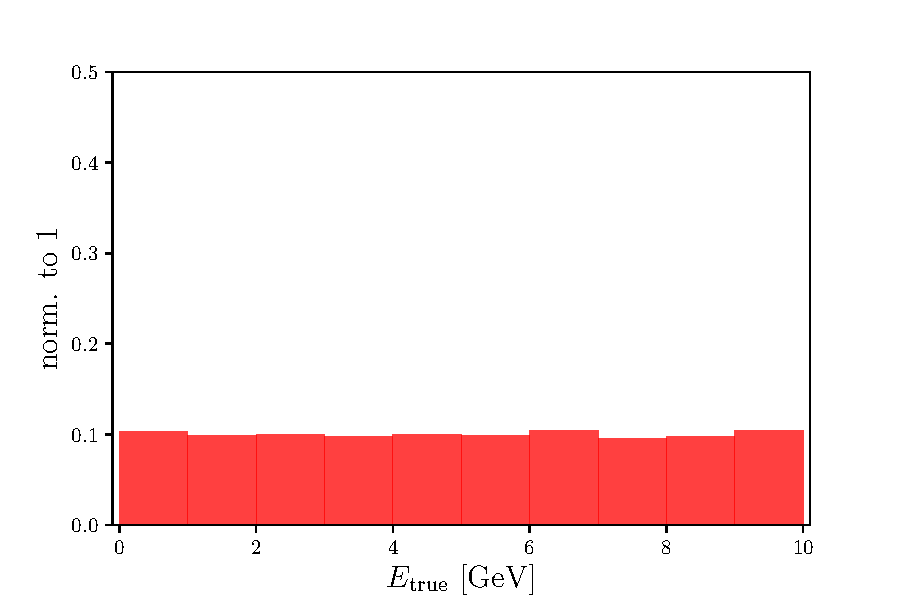
\includegraphics[width=0.8 \textwidth]{../images/energy_distribution.pdf} }
  \caption{\added{The energy distribution of the incoming particles}}%
  \label{fig:e-distr}%
\end{figure}


\begin{figure}[H]%
  \centering
  \subfloat[complete spectrum]{{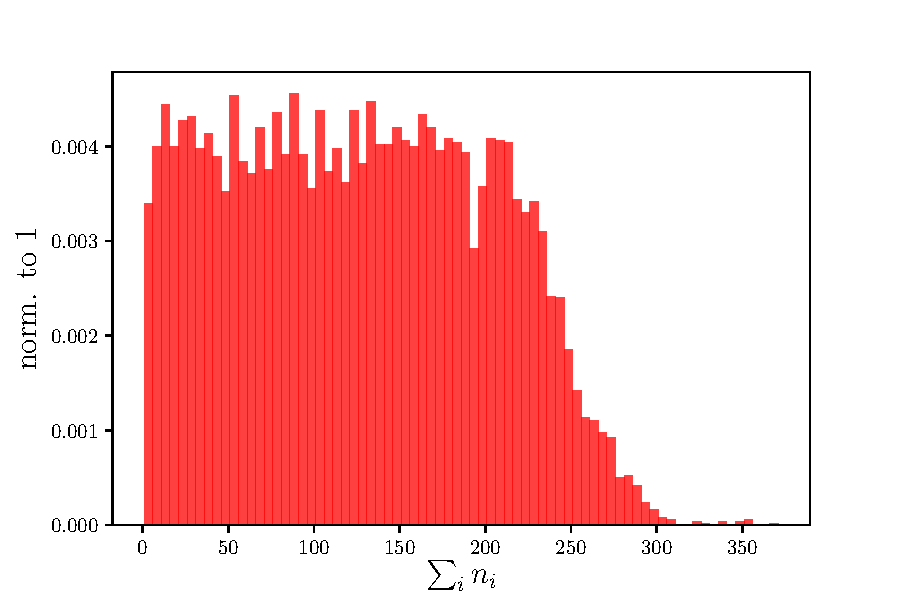
\includegraphics[width=0.45 \textwidth]{../images/sumn_distribution.pdf} }}%
  \qquad
  \subfloat[spectrum at 2 and 8 GeV]{{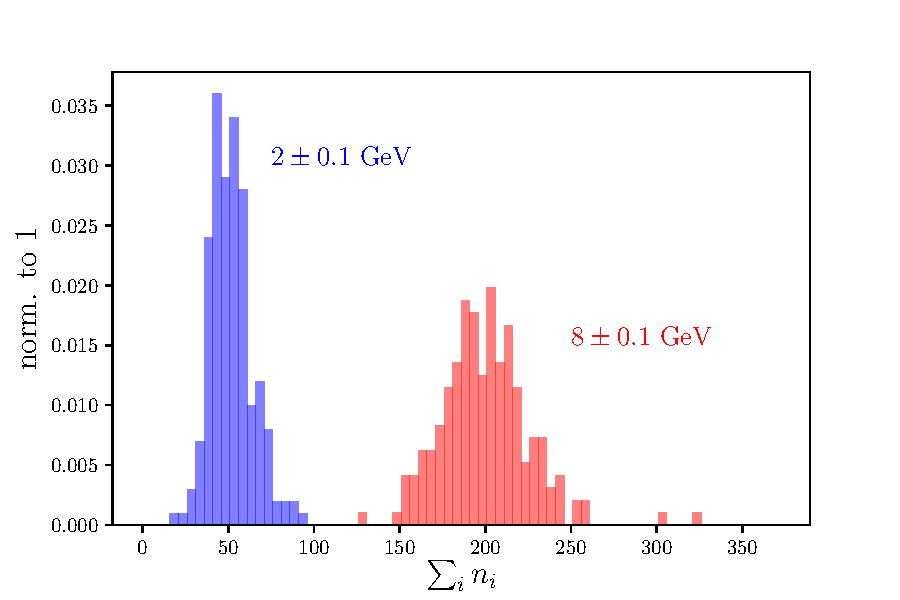
\includegraphics[width=0.45 \textwidth]{../images/sumn_e28_distribution.pdf} }}%
  \caption{\added{Distribution of summed up traced in the calorimeter cells}}%
  \label{fig:n-distri}%
\end{figure}

\added{In the following figures the complete spectrum is shown on the
  left, while on the right two samples from the distribution are
  shown. In this case only values in a range of $2\pm 0.1$ and $8 \pm
  0.1$ GeV are shown.}

\added{The figures \ref{fig:n-distri} show the distribution of the
  total summated traces in the calorimeter cells. Figure
  \ref{fig:n-distri}a shows that the distribution follows the flat
  energy spectrum, only at the end of the distribution the values and
  are no longer uniformly distributed. In \ref{fig:n-distri}b you can
  see that as expected higher energies lead to more traces in the
  detector and their distribution gets wider.}

\begin{figure}[H]%
  \centering
  \subfloat[complete spectrum]{{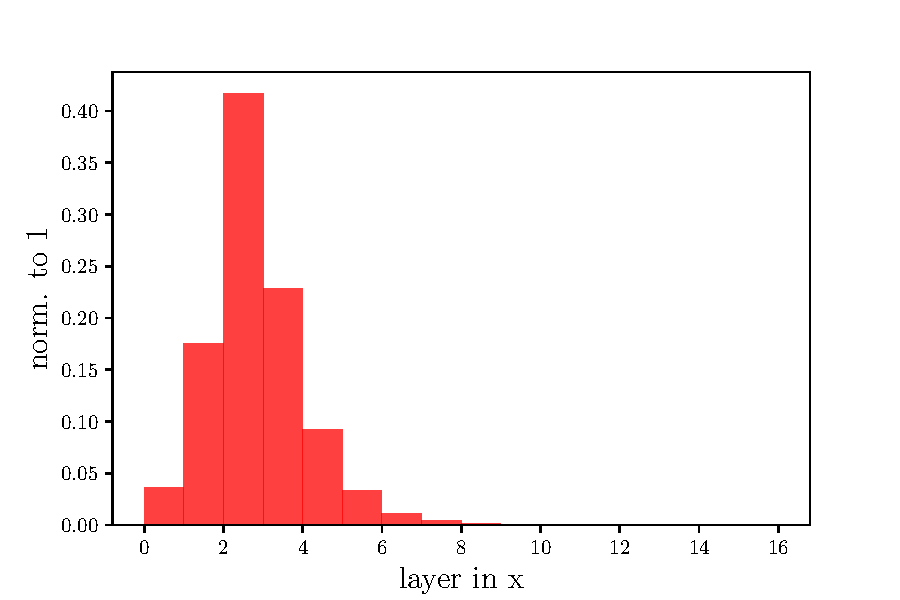
\includegraphics[width=0.4 \textwidth]{../images/x_distribution.pdf} }}%
  \qquad
  \subfloat[spectrum at 2 and 8 GeV]{{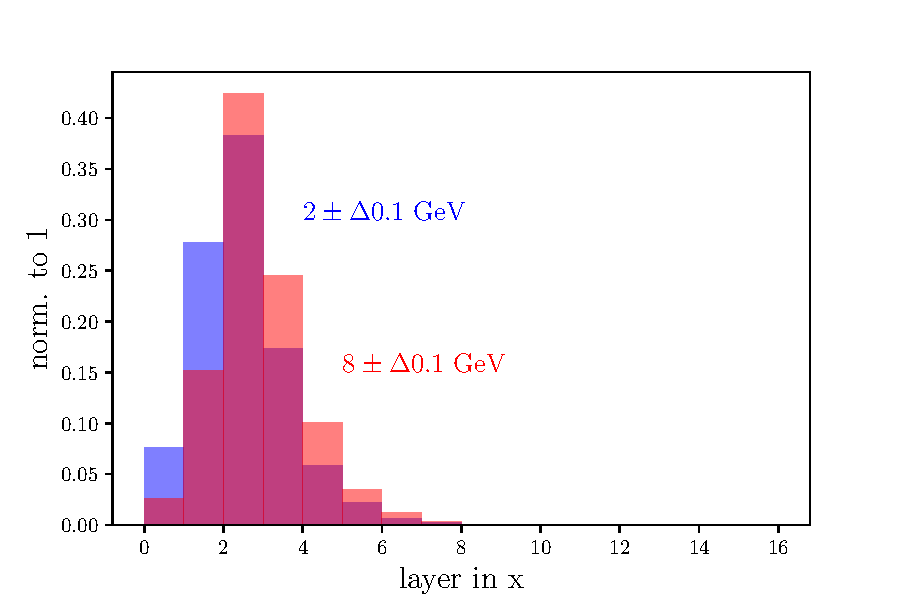
\includegraphics[width=0.4 \textwidth]{../images/x_e28_distribution.pdf} }}%
  \caption{\added{Distribution of summed up traces in the direction of the incoming particle}}%
  \label{fig:x-distri}%
\end{figure}

\added{Figure \ref{fig:x-distri} shows the distribution of the summed traces in the individual layers in the beam direction. \ref{fig:x-distri}a shows that electrons in the selected energy range with the selected calorimeter architecture almost exclusively interact with the first layers. In \ref{fig:x-distri}b you can see that the variation between 2 and 8 GeV electrons is visible in beam direction In \ref{fig:x-distri}b you can see that the variation between 2 and 8 GeV electrons is clearly visible in beam direction but there are no major differences.}

\begin{figure}[H]%
  \centering
  \subfloat[complete spectrum]{{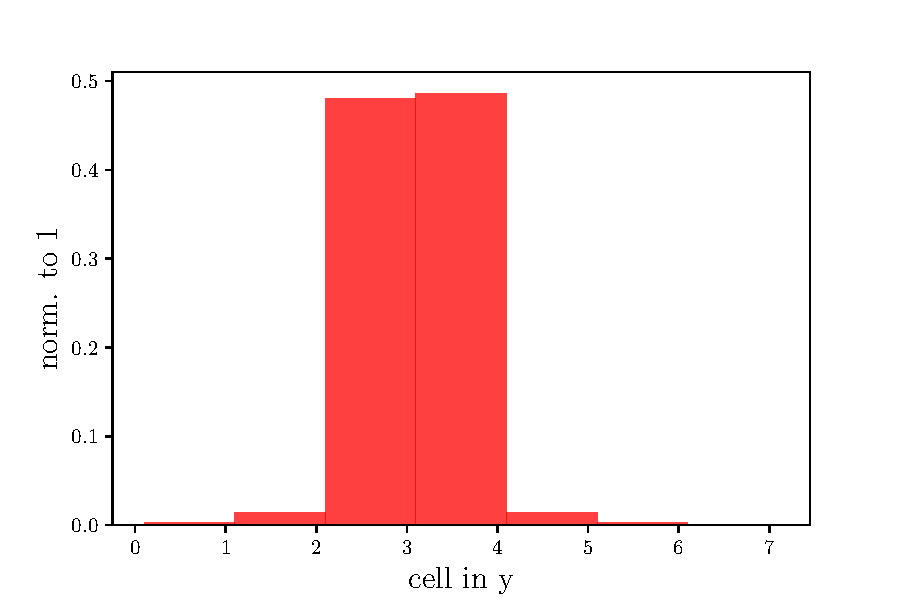
\includegraphics[width=0.4 \textwidth]{../images/y_distribution.pdf}}}%
  \qquad
  \subfloat[spectrum at 2 and 8 GeV]{{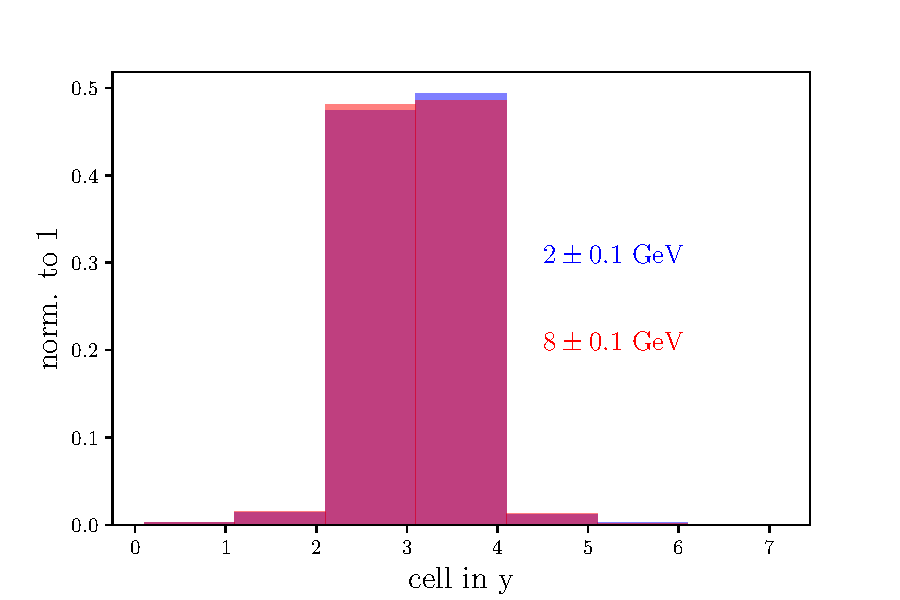
\includegraphics[width=0.4 \textwidth]{../images/y_e28_distribution.pdf} }}%
  \caption{\added{Distribution of summed up traces perpendicular to  the direction of the incoming particle}}%
  \label{fig:y-distri}%
\end{figure}

\added{Figure \ref{fig:y-distri} shows the distribution of the summed traces
  in the individual cells perpendicular to the beam direction. It can be
  seen that there is no energy information perpendicular to the beam
  direction.}

\section{Energy Regression By Linear Fitting}
\label{sec:orgd10286d}

The traditional method of determining the energy of a particle shower
is to sum up the energies of the individual scintillator
cells. This summation can still be influenced by weighting to
compensate for detector effects. The simulation does not determine the
energy in the individual cells but the number of charged traces. This
should be linear to the deposited energy. Detector effects such as
inhomogeneities can also be neglected in a simulation.

To calibrate the calorimeter, the straight line with the smallest mean
square deviation from the data points is determined. Here, the weights
\(c_0, c_1\) of the function

\begin{align}
  N(E) = c_0 \cdot E + c_1
\end{align}

are determined and the straight line is then inverted. The inversion
is necessary to prevent distortions due to the restricted distribution
of the output energy spectrum. The result is shown in Figure
\ref{e-vs-sum_n_fit}.


\begin{figure}[H]
  \centering
  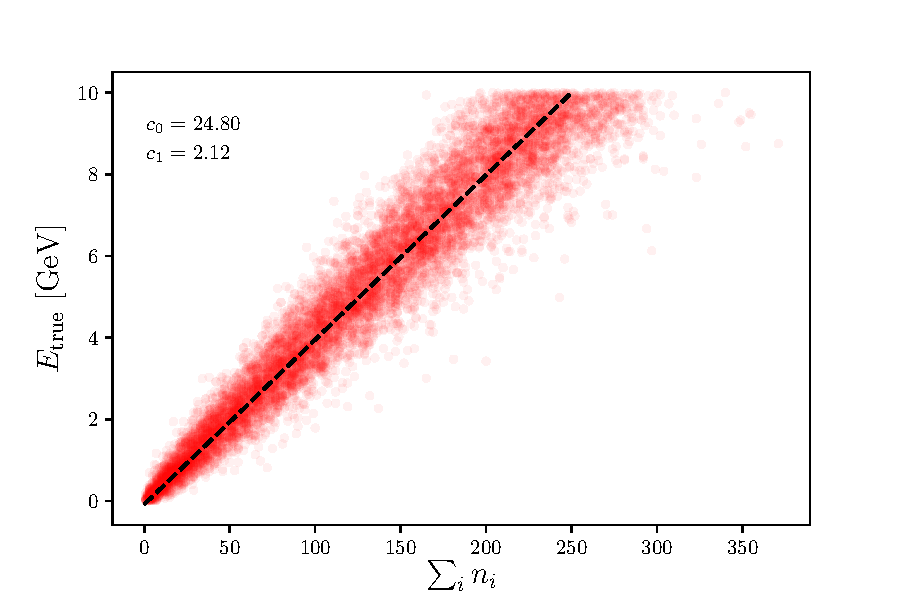
\includegraphics[width=.9\linewidth]{../images/e-vs-sum_n_fit.pdf}
  \caption{ The graph shows the relation between the energies of the
    incoming particle \(E_{\text{true}}\) in GeV and the absolute number
    of charged particles in all scintillator cells.  10000 particles
    from the data are plotted here. The black straight line is the
    result of the fit described above.}
  \label{e-vs-sum_n_fit}
\end{figure}

\section{Fully Connected Setup}
\label{sec:orgb3e1899}

\begin{figure}[H]
  \centering
  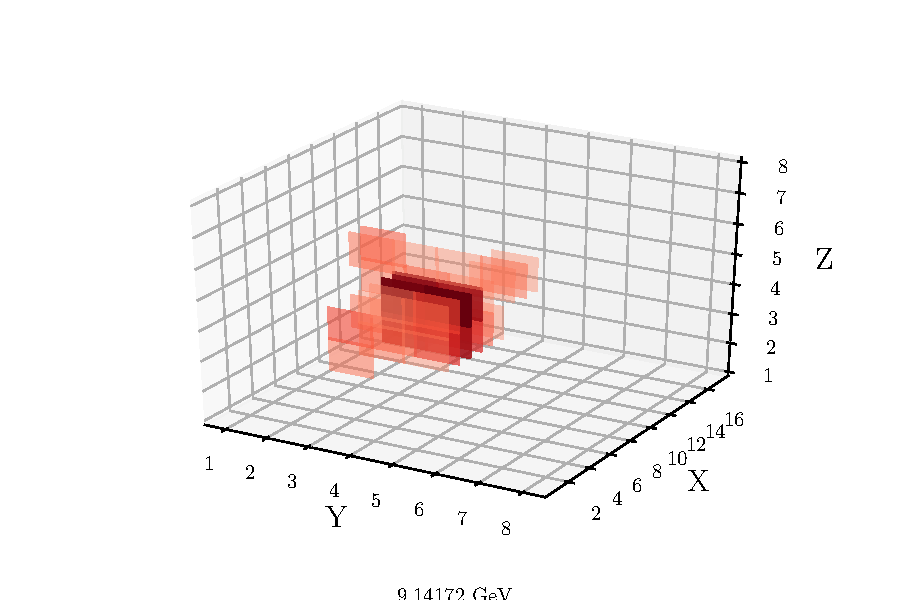
\includegraphics[width=.9\linewidth]{../images/data_display.pdf}
  \caption{The three-dimensional structure of a data sample is
    visulaized by an example event of an incoming electron with
    9.14 GeV}
  \label{data_display}
\end{figure}

The training data set consists of 253,064 simulated events and the
validation set of 28,119 simulated events.

The data structure is visualized in figure \ref{data_display} and is a
three-dimensional pixel structure, where each pixel contains the
number of traces. First a simple fully connected network (FCN) is
applied. % whose structure is not adapted to the structure of the
data.  \added{The data tensor is flatten into a 1088 dimensional
  vector to fit the input space of the FCN}.

%\todo{neural net grafik einfügen}
\begin{table}[H]
  \centering
  \begin{tabular}{lrlr}
    Type & \(\#\) Nodes & Activation & \(\#\) Params\\
    \hline
    FC & 500 & ReLU & 544500\\
    FC & 128 & ReLU & 64128\\
    FC & 128 & ReLU & 16512\\
    FC & 128 & ReLU & 16512\\
    FC & 128 & ReLU & 16512\\
    FC & 10 & ReLU & 1290\\
    FC & 1 & Linear & 11\\
  \end{tabular}
  \caption{The structure of the fully connected network is shown. The
    first column shows the different types of layers of the network,
    \added{which here are only fully connected layers denoted with
      FC}. The second column shows the number of nodes in each
    layer. The third column shows all activation functions and the
    last column shows the number of free parameters or weights of each
    layer.}
  \label{fcn_structure}
\end{table}

The layer structure of the first network is shown in table
\ref{fcn_structure}.  \added{Different structures were tried out. The
  presented version is the one with the best convergence.} It has
659,465 free parameters and each layer \added{is fully connected to
  the previous layer}. With the exception of the output node, all
nodes have ReLU as their activation function. \added{The linear output
  node was choosen to serve the regression task.}

\section{Fully Connected Regression}
\label{sec:orgdf3234b}

The network is trained with the RMSprop optimizer and the loss
function is the mean squared error between the true energy values and
the predicted energy values. The fully connected network is trained
for 150 epochs with a batch size of 128.

\begin{figure}[H]
  \centering
  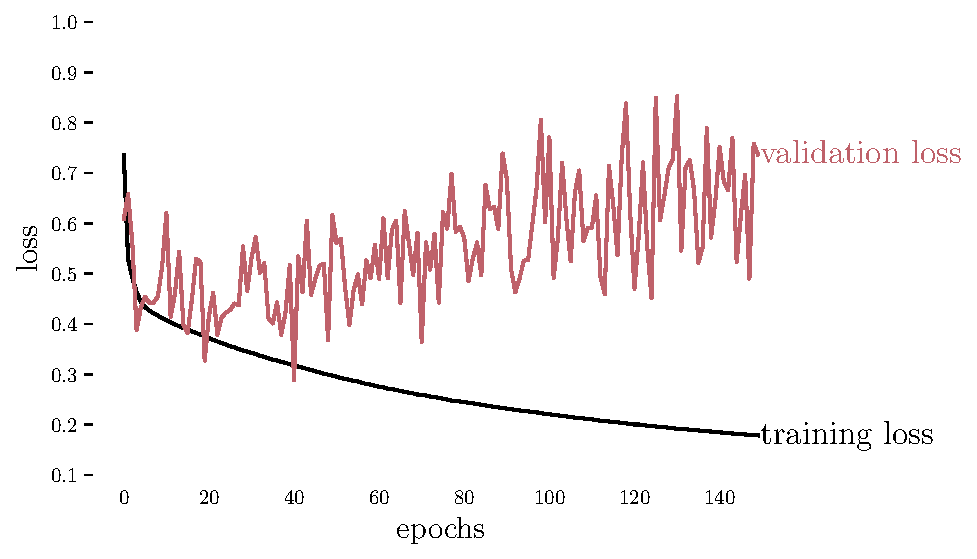
\includegraphics[width=.9\linewidth]{../images/dense_loss.pdf}
  \caption{The Graph shows the evolution of the loss function for the
    training set and the validation set. The trained network was the
    fully connected network described above.}
  \label{dense_loss}
\end{figure}


In figure \ref{dense_loss} the loss function is shown. While the loss
function for the training set decreases over time, the loss function
for the validation set increases. This implies that our model is
overfitting, which means that the model uses the amount of parameters
to remember each point of the data set and not the structure of the
data.

\begin{figure}[H]
  \centering
  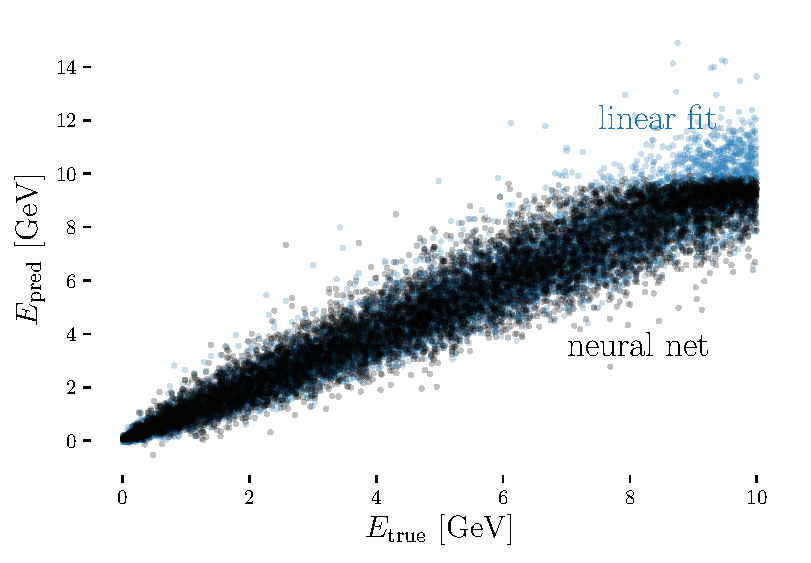
\includegraphics[width=.9\linewidth]{../images/dense_scatter.pdf}
  \caption{ 10000 data points are plotted in a scatter plot between
    \(E_\text{pred}\) and \(E_{\text{true}}\) for the network and the fit. The blue
    background shows the results of the linear fit. In the foreground,
    the results of the fully connected neural net are shown in black.}
  \label{dense_scatter}
\end{figure} 

In the scatter plot in figure \ref{dense_scatter} the results of the
network and the linear fit are compared with each other. Globally the
distributions of the points hardly visibly deviate from each
other. Soley the decrease of the network is visible towards the end of
the distribution.  The network shows hardly any values for
\(E_{\text{pred}}\) above 10 GeV.

\begin{figure}[H]
  \centering
  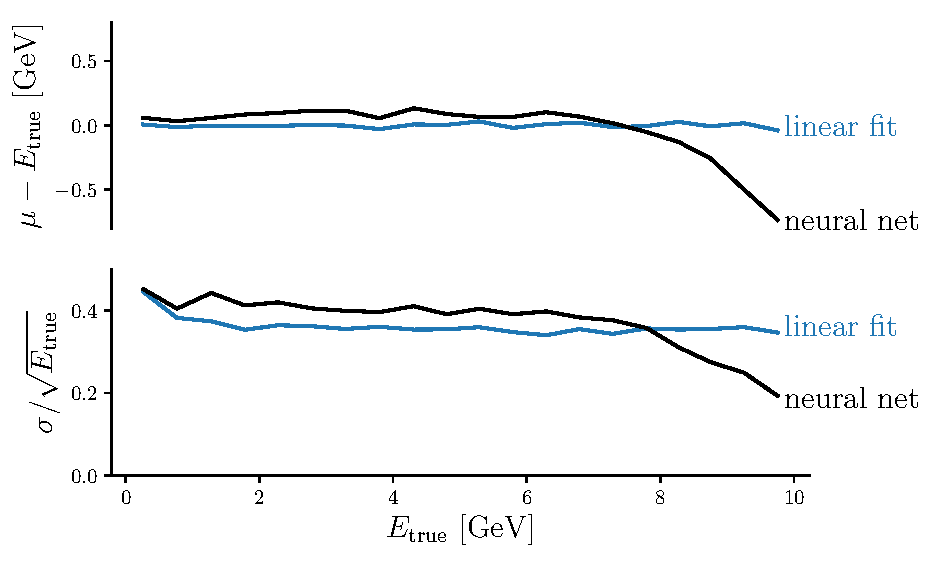
\includegraphics[width=.9\linewidth]{../images/dense_res.pdf}
  \caption{ The results of the neural network and the linear fit are
    compared with each other in the two graphs. The total data points
    were divided into 20 bins and then the mean \(\mu\) and standard
    deviation \(\sigma\) of these bins were calculated. The upper graph
    shows the deviation of the mean values of \(E_{\text{pred}}\) versus the mean
    values of \(E_{\text{true}}\). In the lower plot the standard deviation of \(E_{\text{pred}}\)
    is plotted for each bin divided by the root of the mean
    energy. \added{The graph shows the path from the middle of the first
      to the middle of the last bin.}}
  \label{dense_res}
\end{figure} 

The results of the neural network and the linear fit are compared with each
other in Figure \ref{dense_res}. In the upper plot the decrease of the mean values
of the energies at the edge of the spectrum is visible. In addition, it is
noticeable that the values are slightly shifted upwards globally.

The lower graph shows the dependence of the mean values of the
standard deviations on the root of the energies. The quantity is a
measure for the resolution of the calorimeter, as described in section
\ref{sec:em-calo}. It is noticeable that the global performance of the
neuronal network is weaker than the one of the linear fit. Only at the
end of the distribution is it significantly better than the resolution
of the linear fit.

It can be noted that the FCN optimizes its resolution by respecting
the fact that the distribution is limited between 0 and 10 GeV. The
result is a drop in the value spectrum that is not physically
motivated, but arises solely from the restricted output statistics.
The global shift slightly to higher values is the result of the mean
squared error as a loss function. Thus the residuals of values with
higher energies are greater than those of small energies. The network
therefore optimizes itself to these higher values. Since the network
is overfitted, this is reflected in the poor resolution.

The next section is mainly concerned with solving the problems previously
described.

\section{Data Augmentation}
\label{sec:org4a347fb}

In order to solve the overfitting problem, the technique of data
augmentation was used. In this application data augmentation means
that all valid symmetry transformations were used to increase the
number of data points. Each data point is randomly rotated up to 3
times by 90 degrees and randomly mirrored horizontally. This increases
the possible data points eightfold and should enable the network to
learn the symmetries in the system. The data points were then moved in
every direction discrete in cell size to make the data independent of
their arrival point. At this point it should be noted that these
transformations are only valid because the simulation is absolutely
homogeneous and symmetrical. This is not necessarily the case with
real detector data.

\begin{figure}[H]
  \centering
  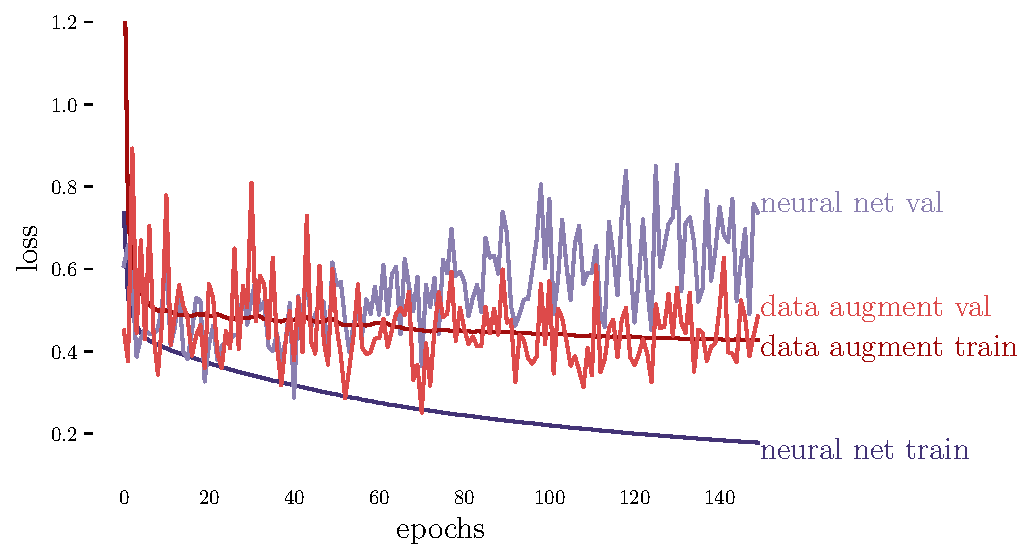
\includegraphics[width=.9\linewidth]{../images/data_augment_loss.pdf}
  \caption{The value of the loss function is shown after each epoch
    for the fully connected network. Val and train stand for the value
    of the loss function on the validation set and the training
    set. Neural net denotes the network without data augmentation,
    while data augmentation stands for the network with data
    augmentation.}
  \label{da_loss}
\end{figure} 

As shown in figure \ref{da_loss}, the overfitting for the dataset can
be completely removed with this method.  The fluctuations in the
values of the loss function for the validation sample result from the
higher statistical fluctuation of a smaller amount of data. With data
augmentation, the global trend follows asymptotically the loss for the
training set. It does not longer show the increase of loss function
for the validation set without data augmentation. This indicates that
the network is not overfitting any longer.

\section{\added{Convolutional Setup}}

To improve the performace of the regression, a convolutional network
is used.

The idea is that since our data has the same structure as images,
techniques used for image recognition should provide improved results.

The network consists of a convolutional part to which a fully
connected network is linked. The layer structure is shown in table
\ref{conv_structure}.

%\todo{struktur-grafik}
\begin{table}[htbp]
  \centering
  \begin{tabular}{lrlr}
    Type & \(\#\) Filter & Activation & \(\#\) Params\\
    \hline
    Conv3D(3,3,3) & 32 & ReLU & 896\\
    Conv3D(3,3,3) & 10 & ReLU & 8650\\
    Conv3D(5,5,5) & 5 & ReLU & 6255\\
    \hline
    Type & \(\#\) Nodes & Activation & \(\#\) Params\\
    \hline
    FC & 128 & ReLU & 28288\\
    FC & 128 & ReLU & 16512\\
    FC & 128 & ReLU & 16512\\
    FC & 10 & ReLU & 1290\\
    FC & 1 & Linear & 11\\
  \end{tabular}
  \caption{The structure of the 3D convolutional network is
    presented. The first column shows the different types of layers of
    the network. The 3D tuples behind the Conv3D are the kernel
    dimensions. The second column shows the number of nodes or filter
    in each layer. The third column shows all activation functions and
    the last column shows the number of free parameters or weights of
    each layer.}
  \label{conv_structure}
\end{table}

The convolutional network has 78,414 free parameters, which are only
12 percent of the parameters of the fully connected network previously
used.

The structure was changed iteratively until the performance of the
network converged.

\section{Adversarial Training}
\label{sec:org30a0273}

In order to reduce the unphysical deviations at the end of the
distribution, an adversarial network is used.

\added{Here the trained network consisted of the convolutional network
  described above as the predictor to which a fully connected network
  is connected as an adversary. The structure of the adversary network
  is shown in Table \ref{adv_structure}}

\begin{table}[htbp]
  \centering
  \begin{tabular}{lrlr}
    Type & \(\#\) Nodes & Activation & \(\#\) Params\\
    \hline
    Dense & 50 & ReLU & 100\\
    Dense & 50 & ReLU & 2550\\
    Dense & 50 & ReLU & 2550\\
    Dense & 50 & ReLU & 2550\\
    Dense & 128& ReLU & 6528\\
    Dense & 20 & Sigmoid & 2580\\ 
  \end{tabular}
  \caption{The structure of adversarial network is presented.}
  \label{adv_structure}
\end{table}


The convolutional network was first pretrained with the mean squared
error as a loss function.

Out of the result of the predictor the quantity

\((E_{\text{pred}}-E_{\text{true}})/\sqrt{E_{\text{true}}}\)

is calculated, which is an approximation for the resolution of a
calorimeter, see section \ref{sec:em-calo}. This quantity is the input
for the adversary which also tries to reconstruct the energy out of
this quantity. The adversary network was trained with Categorial Cross
Entropy as loss function

\begin{align}
\mathcal{L}_r = - \sum \mathcal{C}\left(Y_{\text{true}}\right)
\log(r\left(\frac{f(X)-Y_{\text{true}}}{\sqrt{Y_{\text{true}}}}\right)).
\end{align}

Here \(f\) and \(r\) are the function of the network and its
adversary. \(\mathcal{C}\) is the function that divides all values
from 0. to 10. GeV into 20 categories equal in distance and then maps
each category to a 20-dimensional base vector.

After training the adversary the predictor is trained with the loss
function

\begin{align}
\mathcal{L}_f = \sum (Y_{\text{true}} - f(X))^2 - \lambda
\mathcal{L}_r.
\end{align}

\(\lambda\) is an arbitrary factor that has been set to 2.5 here. This
was choosen so that the gradient of the two parts of the loss function
are nearly equal. By integrating the adversary negatively, the
predictor tries to make the performance of the adversary as poor as
possible. When training the adversary, the weights of the predictor
are locked and vice versa.

The training course consisted of alternative training of both networks
for 5 epochs each. This process was repeated nine times and after each
process the results for the test sample of the neural network were
recorded.

\begin{figure}[H]
\centering
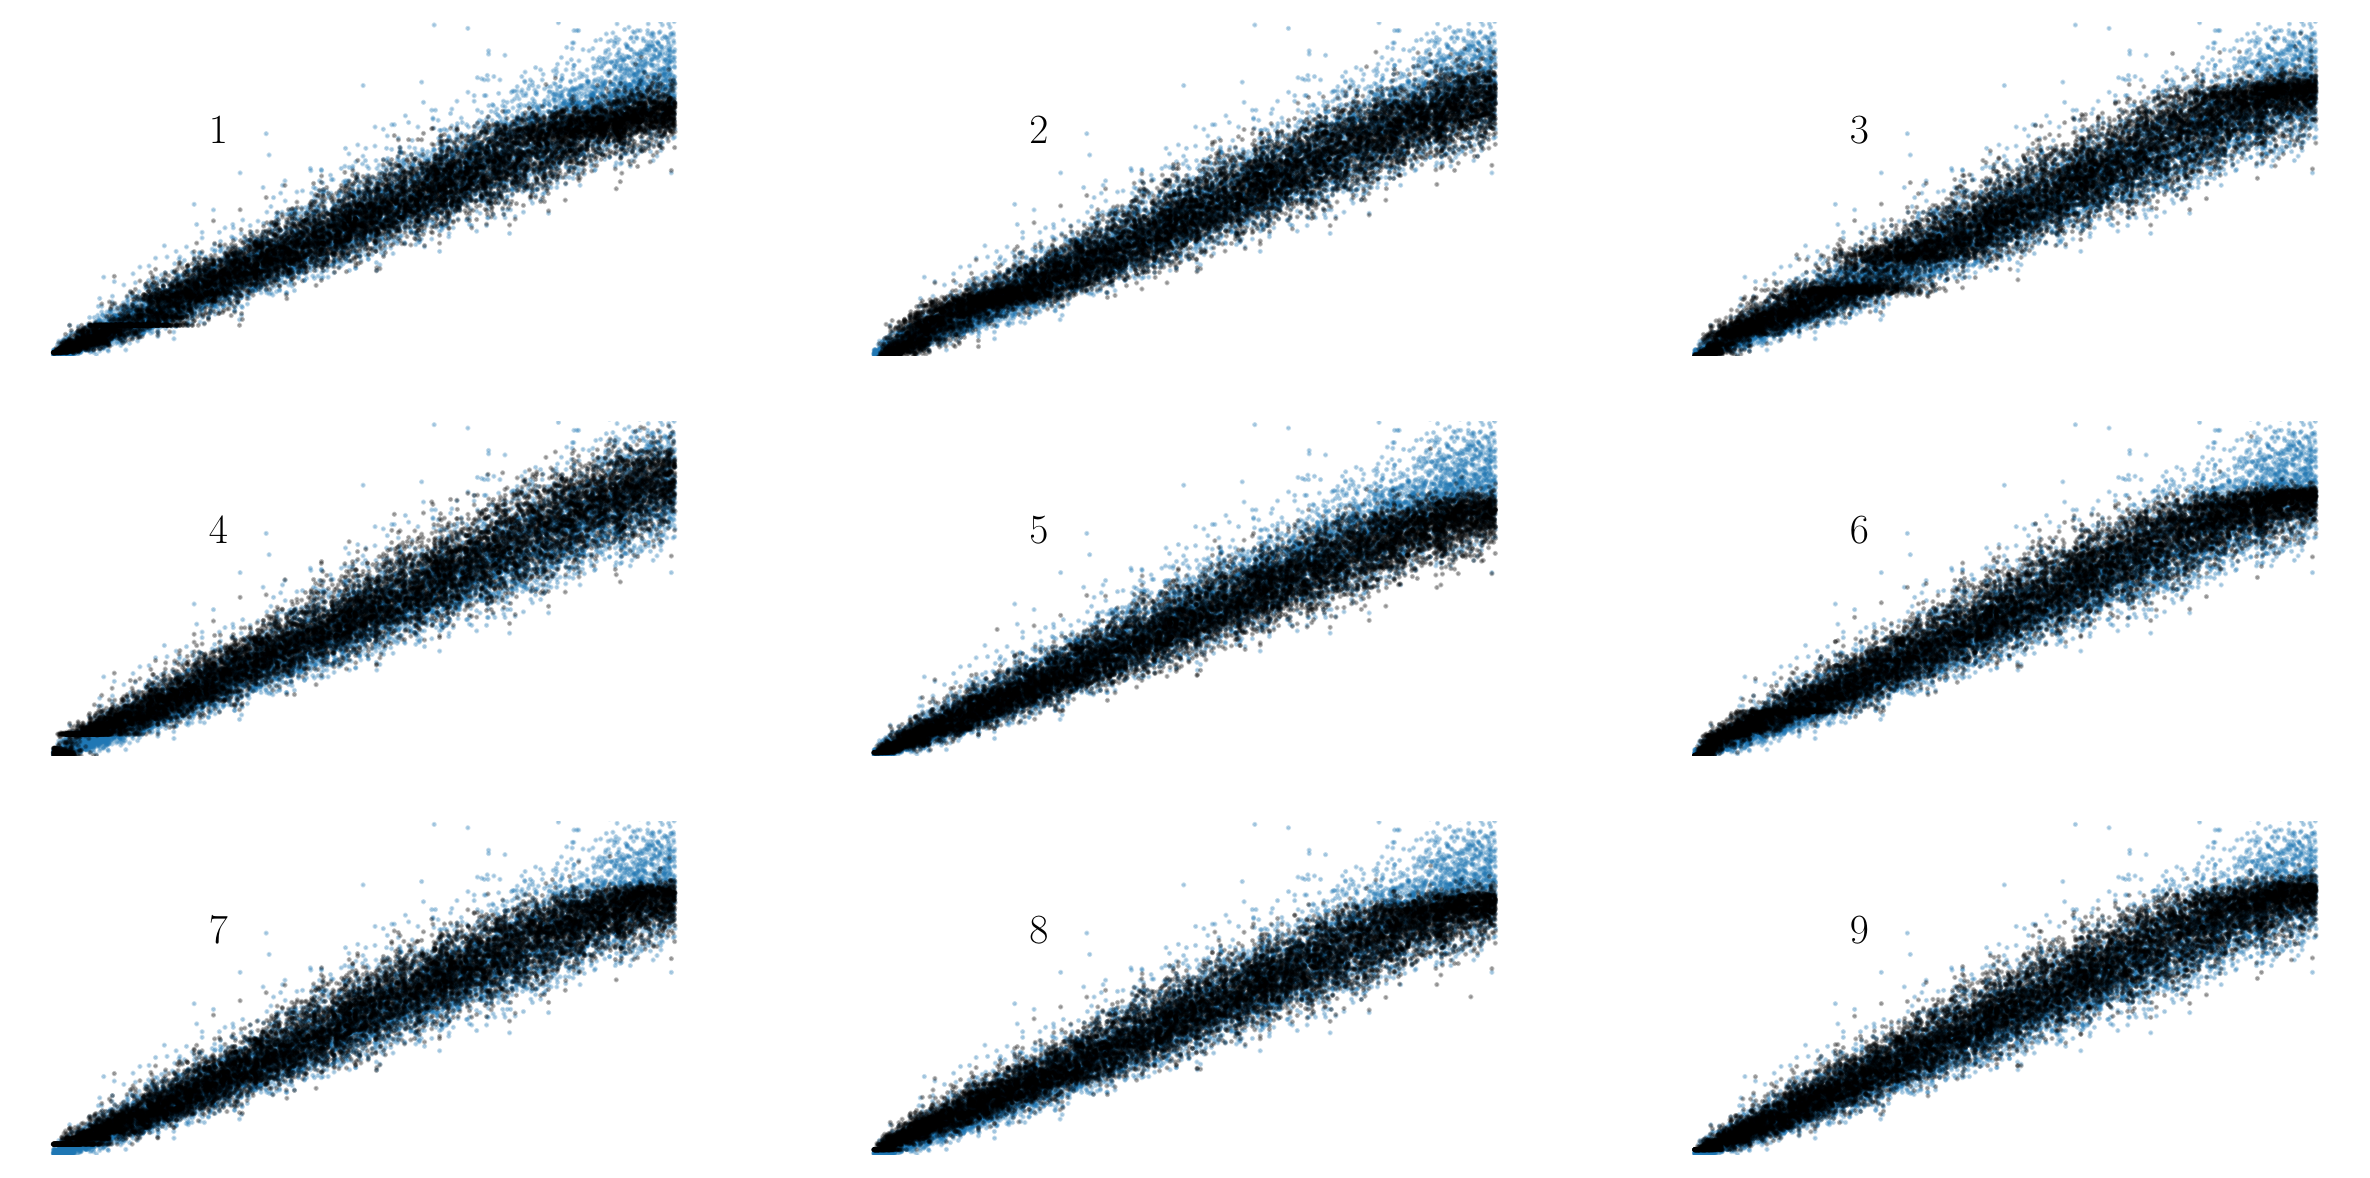
\includegraphics[width=.9\linewidth]{../images/adv_scatter.png}
\caption{ The results of the neural network after every of the 9
  subsequent steps are presented, see numbers. To improve clarity, no
  axes or labels were shown, they are the same as in figure
  \ref{dense_scatter}.}
\label{adv_scatter}
\end{figure}

The results are shown in figure \ref{adv_scatter}.  It is evident that
the results fluctuate and do not converge. With the exception of
anomalies that occur in the meantime, the final result hardly changes
noticeably.

\section{Likelihood Solution}
\label{sec:org05c2ceb}

As the Adversarial Training did not lead to desired results in the
following part the compensation of the deviations in the distribution
by changing the loss function was examined.

Different to the previous parts a modified loss function was used. It
is outlined how an adequate loss function can be determined with
respect to the underlying distribution of labels.

By transforming the mean squared error and adding permissible values,
a maximum likelihood can be derived

\begin{align}
    &\text{min} \sum (y_{\text{true}}-y_{\text{pred}})^2
  \\ =&\text{max} \sum\frac{-(y_{\text{true}}-y_{\text{pred}})^2}{2
    \sigma^2} - \ln(\sqrt{2\pi \sigma^2}) \\ = &\text{max} \sum
  \ln(\exp(-\frac{(y_{\text{true}}-y_{\text{pred}})^2}{2 \sigma^2})) -
  \ln(\sqrt{2\pi \sigma^2}) \\ = &\text{max} \sum \ln(
  \frac{1}{\sqrt{2\pi \sigma^2}}
  e^{-\frac{(y_{\text{true}}-y_{\text{pred}})^2}{2 \sigma^2}}) \\ =
  &\text{max} \ln \prod \frac{1}{\sqrt{2\pi \sigma^2}}
  e^{-\frac{(y_{\text{true}}-y_{\text{pred}})^2}{2 \sigma^2}}\\ =
  &\text{max} \prod \frac{1}{\sqrt{2\pi \sigma^2}}
  e^{-\frac{(y_{\text{true}}-y_{\text{pred}})^2}{2 \sigma^2}}.
\end{align}

The assumption that the mean squared error is the valid minimization
function of the neural network is therefore equivalent to the
assumption that the values are Gaussian distributed and have a
constant standard deviation.

However, no constant standard deviation is given for a calorimeter. In
addition, the assumption that the values have a full Gaussian
distribution is not applicable at the edges. Here the absence of
entries for higher energies must be compensated with a normalization
factor. To illustrate this in figure \ref{gaussian-cut} random values
normal distributed with a mean of 9.5 and a standard deviation of
$\sqrt{9.5}$ are shown. All values of the random sample above 10 are
dropped. To this data points two maximum likelihood fits are
applied. One for a gaussian distribution and one for a gaussian
distribution divided by the cumulitive gaussian distribution at 10,

\begin{align}
\frac{\frac{1}{\sqrt{2\pi \sigma^2}} e^{-\frac{(x-\mu)^2}{2
      \sigma^2}}}{\int^{10}_{-\infty} \frac{1}{\sqrt{2\pi \sigma^2}}
  e^{-\frac{(x-\mu)^2}{2 \sigma^2}} \dd x}.
\end{align}

\begin{figure}[H]
  \centering
  \includegraphics[width=.9\linewidth]{../images/gaussian_cut.pdf}
  \caption{The data shown are random values normal distributed with a
    mean of 9.5 and a standard deviation of $\sqrt{9.5}$. All values
    above 10 is excluded. The two lines are gaussians fitted with a
    maximum likelihood fit to the data. The black line gaussian is a
    standard gaussian and the blue line is a gaussian divided by a
    normalization compensating for the missing values above 10.}
  \label{gaussian-cut}
\end{figure}


It is visible that without this normalization the distribution is
shifted and not resembles the data. So in order to consider truncated
distributions the probability density function can be calculated as

\begin{align}
\frac{\frac{1}{\sqrt{2\pi \sigma^2}}
  e^{-\frac{(x-\mu)^2}{2 \sigma^2}}}{\int^b_a \frac{1}{\sqrt{2\pi
      \sigma^2}} e^{-\frac{(x-\mu)^2}{2 \sigma^2}} \dd x} =
\frac{\frac{1}{\sqrt{2\pi \sigma^2}} e^{-\frac{(x-\mu)^2}{2
      \sigma^2}}}{1/2\left(\text{erf}\left(\frac{\mu-a}{\sqrt{2}\sigma}\right)
  - \text{erf}\left(\frac{\mu-b}{\sqrt{2}\sigma}\right)\right)},
\end{align}

where \(a\) and \(b\) in the simulation are 0.0 and 10.0 GeV. A loss
function which has to be minimized for the neural net can than be
derived as

\begin{align}
&\text{max}\left[ \prod \frac{\frac{1}{\sqrt{2\pi \sigma^2}}
      e^{-\frac{(x-\mu)^2}{2
          \sigma^2}}}{1/2\left(\text{erf}\left(\frac{\mu-a}{\sqrt{2}\sigma}\right)
      - \text{erf}\left(\frac{\mu-b}{\sqrt{2}\sigma}\right)\right)}
    \right]\\ &=\text{min}\left[ -\ln \prod \frac{\frac{1}{\sqrt{2\pi
          \sigma^2}} e^{-\frac{(x-\mu)^2}{2
          \sigma^2}}}{1/2\left(\text{erf}\left(\frac{\mu-a}{\sqrt{2}\sigma}\right)
      -
      \text{erf}\left(\frac{\mu-b}{\sqrt{2}\sigma}\right)\right)}\right]
  \\ &=\text{min}\left[ -\sum \ln(e^{-\frac{(x-\mu)^2}{2
        \sigma^2}}{\sqrt{\frac{\pi
          \sigma^2}{2}}\left(\text{erf}\left(\frac{\mu-a}{\sqrt{2}\sigma}\right)
      -
      \text{erf}\left(\frac{\mu-b}{\sqrt{2}\sigma}\right)\right)})\right]
  \\ &=\text{min}\left[ -\sum -\frac{(x-\mu)^2}{2
      \sigma^2}-\ln(\sqrt{\frac{\pi
        \sigma^2}{2}}\left(\text{erf}\left(\frac{\mu-a}{\sqrt{2}\sigma}\right)
    -
    \text{erf}\left(\frac{\mu-b}{\sqrt{2}\sigma}\right)\right))\right]
  \\ &=\text{min} \sum \frac{(x-\mu)^2}{\sigma^2} + \ln(\frac{\pi
    \sigma^2}{2}\left(\text{erf}\left(\frac{\mu-a}{\sqrt{2}\sigma}\right)
  -
  \text{erf}\left(\frac{\mu-b}{\sqrt{2}\sigma}\right)\right)^2). \label{likelihood-loss}
\end{align}


The resulting loss function consists of a mean weighted squared term
part and a boundary correction term. This weighting prevents the
global shift of the mean $\mu$ towards higher values. Because values
with high energies contribute to the total loss function the same
amount as values with low energies. The second term is a correction
factor that takes into account the ends of the distribution and
reduces its effects.

\added{Convergence problems occurred with the resulting loss function
  when the selected initial parameters were far from the
  optimum. Therefore the network was pre-trained with the MSE until it
  converged.}  The pre-trained ConvNet was then further trained with
\eqref{likelihood-loss} as loss function for 50 epochs. The result is
shown in figure \ref{likelihood_res}. The decrease of the mean values
to high energy values was completely removed. Globally, the network
has no tendency to higher values.

\begin{figure}[H]
  \centering
  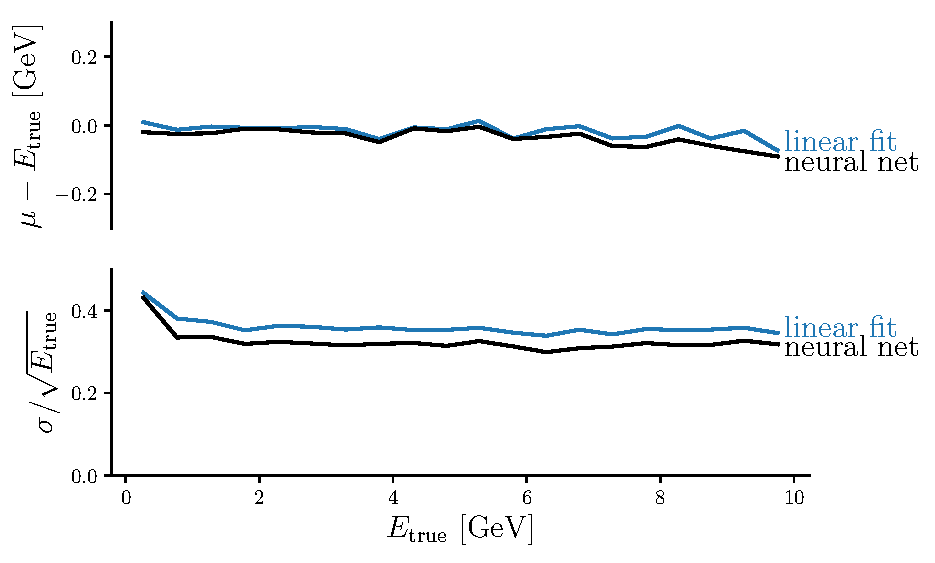
\includegraphics[width=.9\linewidth]{../images/likelihood_res.pdf}
  \caption{ The results of the neural network and the linear fit are
    compared in the two graphs. The total data points were divided into
    20 bins and then the mean and standard deviation of these bins were
    calculated. The upper graph shows the deviation of the mean values
    of \(E_{\text{pred}}\) versus the mean values of \(E_{\text{true}}\). In the lower plot the
    standard deviation of \(E_{\text{pred}}\) is plotted for each Bin divided by the
    root of the mean energy.}
  \label{likelihood_res}
\end{figure}

\section{Comparison of Network Architectures}
\label{sec:org1df3a0b}

Finally, the performance of the two network architectures, the ConvNet
and the FCN are compared with each other. Both networks were treated
equally. Both the ConvNet and the FCN were each trained 150 epochs
with mean squared error and data augmentation. Afterwards both
networks were trained 50 epochs with the likelihood loss to solve the
boundary problems.

\begin{figure}[H]
  \centering
  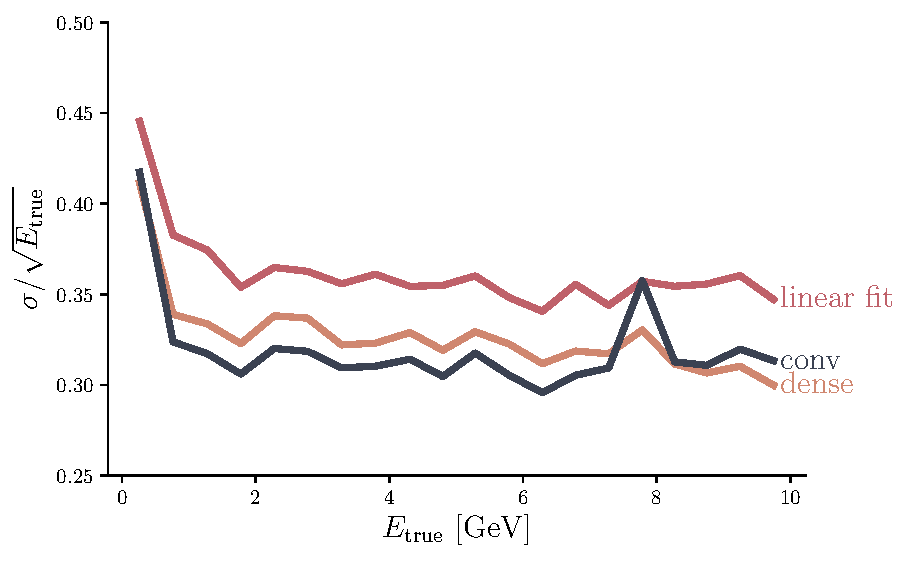
\includegraphics[width=.9\linewidth]{../images/arch_comparison.pdf}
  \caption{ The results of the linear fit, the FCN and the ConvNet are
    compared. The standard deviation of \(E_{\text{pred}}\) is plotted
    for each bin divided by the root of the mean energy.}
  \label{arch_comparison}
\end{figure}

Figure \ref{arch_comparison} shows the different resolutions of the
linear fit, the ConvNet and the FCN. The linear fit performed a mean
resolution of 0.362 $\sqrt{E}$, the FCN of 0.327 $\sqrt{E}$ and the
ConvNet of 0.319 $\sqrt{E}$. With the ConvNet the resolution can be
improved by almost 12 percent.

It should be noted that only the basic possibility of improvement is
presented here. It is beyond the focus of this work to show how much
the resolution can be improved.

\added{Altogether it could be shown that a better resolution for
  calorimeters can be achieved with deep learning. Even if the
  information density in the structure of the data is not high. The
  effectiveness of data augmentation to eliminate overfitting could be
  demonstrated. Adversarial training was not successful. A method
  could be described how a corresponding loss function could be
  derived from the distribution of the values. It could be shown how
  otherwise occurring systematic errors could be eliminated with
  utilising this loss function. The comparison of ConvNet and FCN
  could also show that a network architecture suitable for the data
  leads to better results.}

\chapter{Jet Calibration Analysis}
\label{sec:org03a9b39}

\todo{which jet algo?}
\todo{analyse ablauf plan}
In this chapter, the jet transverse momentum calibration using deep
learning is discussed. The application of the previous methodology for
the reduction of boundary effects on jets is presented. In addition to
a simple network architecture, a particle flow network is also used
for regression.

In this analysis, data generated by the fully detailed Geant
simulation of the CMS detector were used. The data sample used is a
QCD data set belonging to the 2018 detector simulation. The data set
has a \(P_T\) spectrum from 15 to 3000 GeV. The events generated in
the data set were created without pile up.

Individual jets were extracted from the data set for analysis. Only
jets in the energy range between 30 and 150 GeV were selected. The
distribution of the jets is shown in figure \ref{jet_distri}. The
distribution is not flat, but shows the characteristic falling
distribution resulting from the convolution of parton density function
and matrix elements. For this reason the shape of this distribution
must be taken into account in contrast to the last chapter.

\begin{figure}[H]
  \centering
  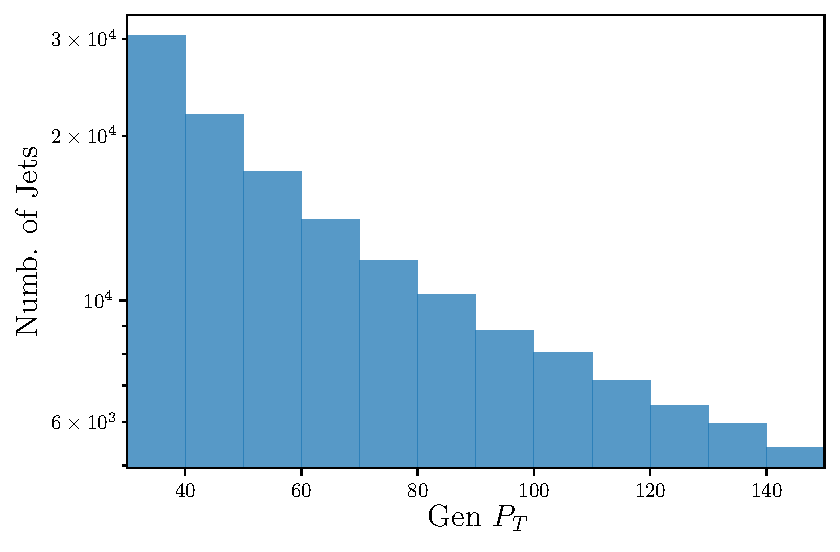
\includegraphics[width=.9\linewidth]{../images/jet_distri.pdf}
  \caption{ The distribution of the jets versus \(P_T\) on generator
    level is plotted for the validation set.}
  \label{jet_distri}
\end{figure}

In total the training set consists of 14,786,472 jets which were
divided into a training set of 14,490,070 jets. The validation set
consisted of 148,318 jets and the test sample 148,084 jets.

The four-vectors of the constituent particle flow objects were stored
for each jet. The transversal momenta of the jets were recorded at
generator level and after simulation. For each jet, only a maximum of
200 four-vectors sorted by transverse momentum were stored. In order
to obtain a constant input size. When a jet consisted of less than 200
particles, the free entries were filled with zero vectors.

\section{Deep Learning Setup}
\label{sec:orgf3b24cc}





\begin{figure}[H]
  \centering
  \tikzset{
    %Define standard arrow tip
    >=stealth',
    %Define style for boxes
    punkt/.style={
      rectangle,
      draw=black, thick,
      text width=6.5em,
      minimum height=2em,
      text centered},
    % Define arrow style
    pil/.style={
      ->,
      thick,
      shorten <=2pt,
      shorten >=2pt},
  }
  \begin{tikzpicture}[node distance=0.5cm, auto,]
    %nodes
    \node[punkt] (model) {Model};
    \node[below=2.5cm of model] (1loss) {$\mathcal{L}_{J}(\hat Y, Y, \sigma(Y, c_{0,1,2}))$};
    \node[below=of 1loss] (1st) {1st};
    \node[left=2.5cm of 1loss] (mseloss) {$\mathcal{L}(\hat Y, Y)=(\hat Y - Y)^2$};
    \node[below=of mseloss] (mse) {MSE};
    \node[right=2.5cm of 1loss] (2loss) {$\mathcal{L}_{J}(\hat Y, Y, \sigma(Y, c_{0,1,2}))$};
    \node[below=of 2loss] (2nd) {2nd};

    \draw[->, thick,] (mseloss)  --  (model.south west);
    \node[above right=1.cm and 1.5cm of mseloss.center, rotate=30] (t1) {train};

    \draw[->, thick,] (model.south west) -- (1loss);
    \node[above left=0.3cm and 1.cm of 1loss.center, rotate=-60] (p1) {predict $\sigma$};
    
    \draw[->, thick,] (1loss)  --  (model.south);
    \node[above right=1.cm and 0.5cm of 1loss.center, rotate=90] (t2) {train};

    \draw[->, thick,] (model.south) -- (2loss);
    \node[above left=0.9cm and 3.5cm of 2loss.center, rotate=-25] (p1) {predict $\sigma$};

    \draw[->, thick,] (2loss)  --  (model.south east);
    \node[above left=1.5cm and 2.5cm of 2loss.center, rotate=-35] (t2) {train};

    
\end{tikzpicture}
  \caption{\todo{XXXX}}}
    \label{\todo{XXXX}}
\end{figure}

To deduce the momentum, the 4 vectors of the particles of the jets
were used as an input for the networks. First, the dimensions of the
\((200, 4)\) input space are transformed into a (800, 1) space. The
network is than applied.

The network used for analysis is a very simple fully connected
network.  Table \ref{jet_fcn_structure} shows the structure. The
number of nodes is reduced for each layer.  The first layer has 800
nodes, which corresponds to the number of input features of one
jet. The 7 layers have the ReLU activation function. The last layer
has a linear node to get a linear one-dimensional output space. In
total the network has 2,043,201 free parameters. This network is
referred to as \emph{JetNet} in the following.

\begin{table}[H]
  \centering
  \begin{tabular}{lrlr}
    Type & \(\#\) Nodes & Activation & \(\#\) Params\\
    \hline
    Dense & 800 & ReLU & 640800\\
    Dense & 700 & ReLU & 560700\\
    Dense & 600 & ReLU & 420600\\
    Dense & 400 & ReLU & 240400\\
    Dense & 300 & ReLU & 120300\\
    Dense & 200 & ReLU & 60200\\
    Dense & 1 & Linear & 201\\
  \end{tabular}
  \caption{The structure of the fully connected network is shown. The
    first column shows the different types of layers of the
    network. The second column shows the number of nodes in each
    layer. The third column shows all activation functions and the
    last column the number of free parameters or weights of each
    layer.}
  \label{jet_fcn_structure}
\end{table}

In the training process, the data was processed in batch sizes of
1024. As a first step the network was trained with the mean squared
error as loss function.

Since the data spectrum covered only a limited space of \(P_{T,
  \text{Gen}}\), it was to be expected that the systematic deviations
described in the previous chapter would occur. The fact that the
information from the calorimeters is incorporated into the
reconstructed particles is also correlated with their error structure.

Therefore the loss function from the previous chapter was used. Since
the standard deviation \(\sigma\) was not a priori apparent, it was
approximated before.

For this purpose the results of the network were calculated and
divided into 20 bins according to \(P_{T, \text{Gen}}\). The standard deviation
was then determined for each bin and the analytical function 

\todo{plot fit}
\begin{align}
\sigma(P_{T, \text{Gen}})= c_0 \sqrt{P_{T, \text{Gen}}}+c_1 P_{T, \text{Gen}} + c_2
\end{align}

was fitted to these \(\sigma\) values. This function is used as a
\(\sigma\) term in the loss function. At this point it should be noted
that a differentiable function for \(\sigma\) is indispensable, since
the gradient of the loss function is required for the backpropagation
algorithm. \todo{the initial values for $c_{0,1,2}$ were optained by
  ...} The calculation of the \(\sigma\) values is be done
iteratively. Here this process was iterated twice and the results were
marked with \texttt{1st} and \texttt{2nd}.

\todo{MSE, 1st, 2nd beschreiben}

Since the distribution of the \(P_{T, \text{Gen}}\) values is not
flat, the loss function was divided into equal areas in a further
step.

\todo{neu: This means that the data points were sorted by
  \(P_{T,\text{Gen}}\) and the mean value for each bin was
  calculated. Then the mean value of previously determined mean values
  is used as the loss function value.} As a result, the individual
value ranges in the spectrum no longer contributed to the total value,
even if their population is higher. The bias to values with a high
population will be reduced in this way.

The response \(R\) was used as a measure for the calibration,

\begin{align}
R = \frac{P_{T, \text{Reco}}}{P_{T, \text{Gen}}}.
\end{align}

\section{Jetnet Analysis}
\label{sec:org03235a3}

\begin{figure}[H]
  \centering
  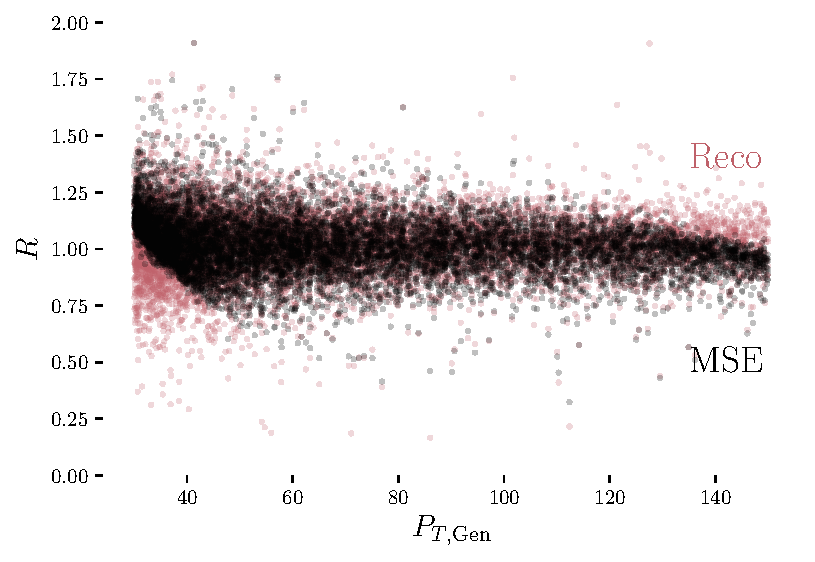
\includegraphics[width=.9\linewidth]{../images/jetnet_R_scatter.pdf}
  \caption{The resulting \(R\) points of the Reco algorithm and the
    Jetnet in relation to \(P_{T, \text{Gen}}\) are displayed.}
  \label{jetnet_R_scatter}
\end{figure}

Figure \ref{jetnet_R_scatter} shows the results of the Reco algorithm
and the neural network in a scatter plot. MSE was used as loss
function for the neural network. The systematic deviations similar to
the previous chapter can be seen at low and high values of \(P_{T,
  \text{Gen}}\).

 
\begin{figure}[H]
  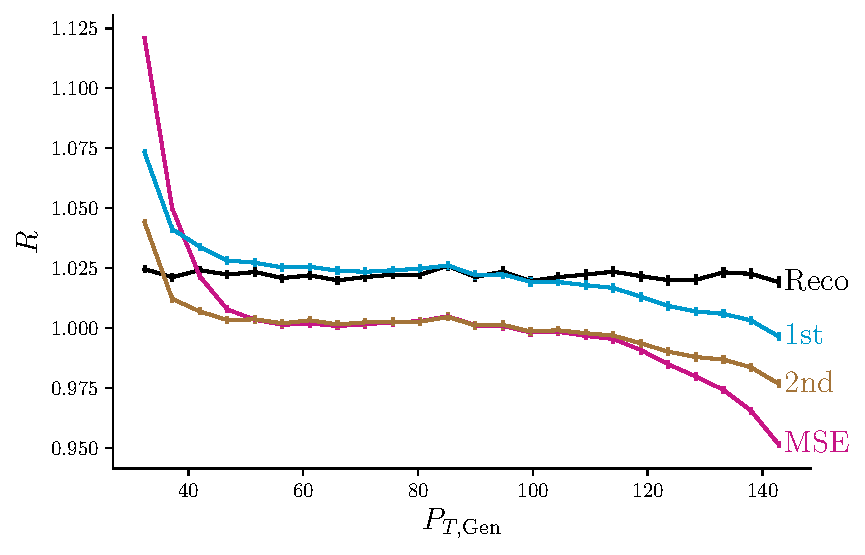
\includegraphics[width=.9\linewidth]{../images/jetnet_R.pdf}
  \caption{The mean values of the R distribution are represented as a
    function of \(P_{T, \text{Gen}}\). Reco stands for the Reco
    algorithm. MSE for the jetnet with MSE as loss function. 1st and
    2nd stand for the first and second iteration with the loss
    function described above.}
  \label{jetnet_R}
\end{figure}

Figure \ref{jetnet_R} shows the mean resulting R values in bin of
\(P_{T, \text{Gen}}\) for the Jetnets and the Reco algorithm. It can
be seen that the first iteration corrects the systematic deviations at
the boundaries, but yields too high results. This shift to higher
values is not found after the second iteration. The boundary effects
could not be removed completely and persist even after multiple
iterations.

\begin{figure}[H]
  \centering
  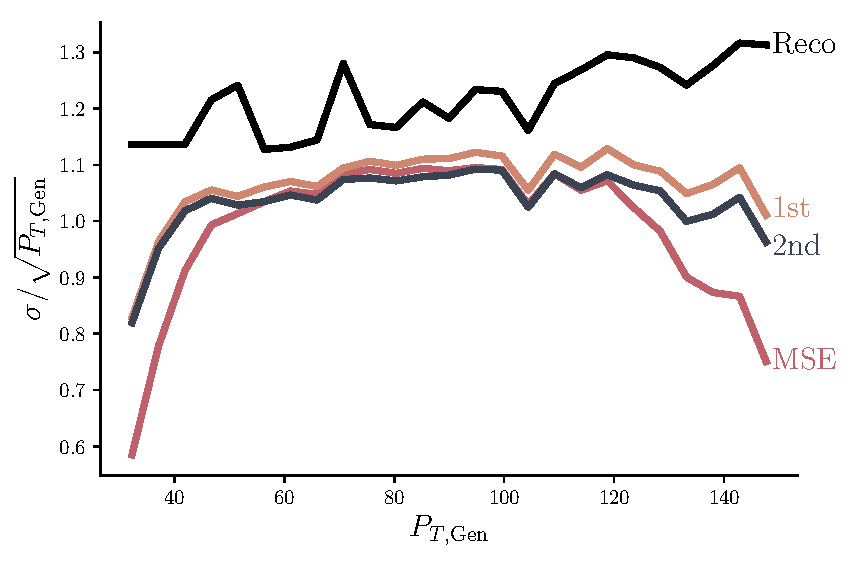
\includegraphics[width=.9\linewidth]{../images/jetnet_res.pdf}
  \caption{ The standard deviation by the root of \(P_{T, \text{Gen}}\)
    in relation to \(P_{T, \text{Gen}}\) is represented.}
  \label{jetnet_res}
\end{figure}

In figure \ref{jetnet_res} the resolution is shown. You can see that all
Jetnets perform better than the Reco algorithm. At the edges the
resolution increases again artificially. This systematic deviation
could be reduced by the alternative loss function.

\section{Particle Flow Network}
\label{sec:org307355e}

Subsequently, a Particle Flow Network (PFNet) was trained for
comparison. To create the network the \texttt{EnergyFlow} packet was used
\cite{komiske19_energ_flow_networ}. The training procedure was the same
as for the Jetnet. The structure of the PFNet consists of a filter
module consisting of three layers with 100, 100 and 128 nodes. So the
latency space was 128 dimensional. The second network consisted of
three layers of 100 nodes each followed by a linear output node.

\begin{figure}[H]
  \centering
  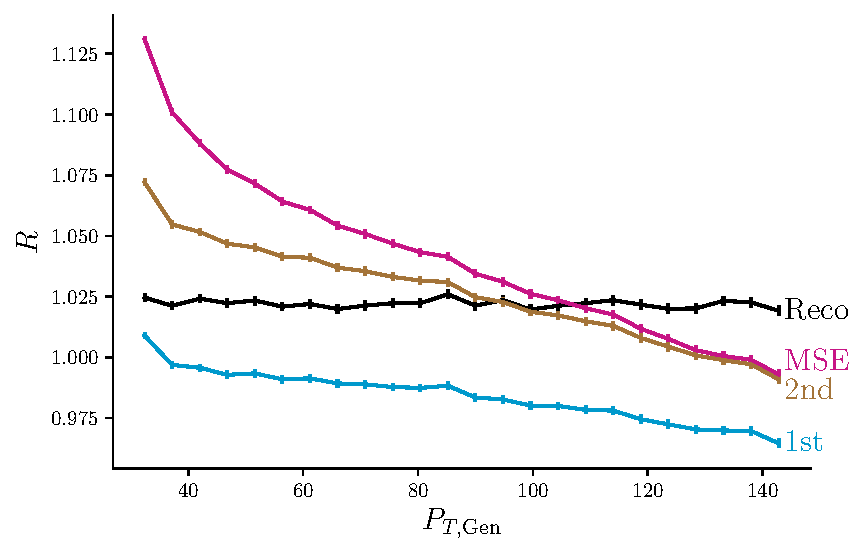
\includegraphics[width=.9\linewidth]{../images/pfnet_R.pdf}
  \caption{The mean values of the R distribution are represented as a
    function of \(P_{T, \text{Gen}}\). Reco stands for the Reco
    algorithm. MSE for the PFNet with 'mse' as loss function. 1st and
    2nd stand for the first and second iteration with different loss
    function.}
  \label{pfnet_R}
\end{figure}

Figure \ref{pfnet_R} shows the mean values of the R
distribution. The results are very similar to those of the Jetnet. You
can see that the alternative loss function helps to eliminate the kink
at the beginning.  Overall the entire distribution has a systematic
skewness, but is quite linear.

\begin{figure}[H]
  \centering
  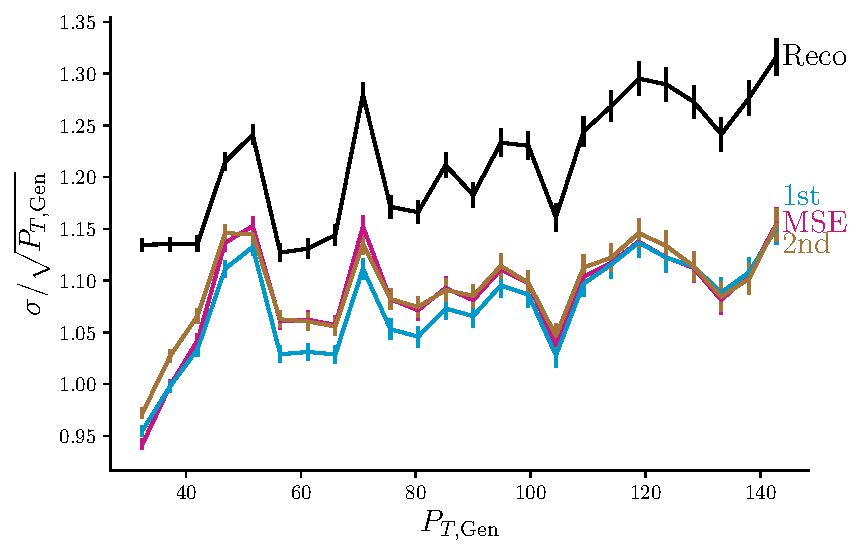
\includegraphics[width=.9\linewidth]{../images/pfnet_res.pdf}
  \caption{The standard deviation by the root of \(P_{T, \text{Gen}}\)
    in relation to \(P_{T, \text{Gen}}\) is shown.}
  \label{pfnet_res}
\end{figure} 

In \ref{pfnet_res} the distribution of the resolutions is shown. All
PFNet results have approximately the same progression and are clearly
below the Reco results. The best performance is achieved after the
second iteration.

\section{Comparison}
\label{sec:org638f190}

The last paragraph compares the two networks. In Fig. \ref{comp_R} it
can be seen that the R distribution of the two network types is almost
identical.

\begin{figure}[H]
  \centering
  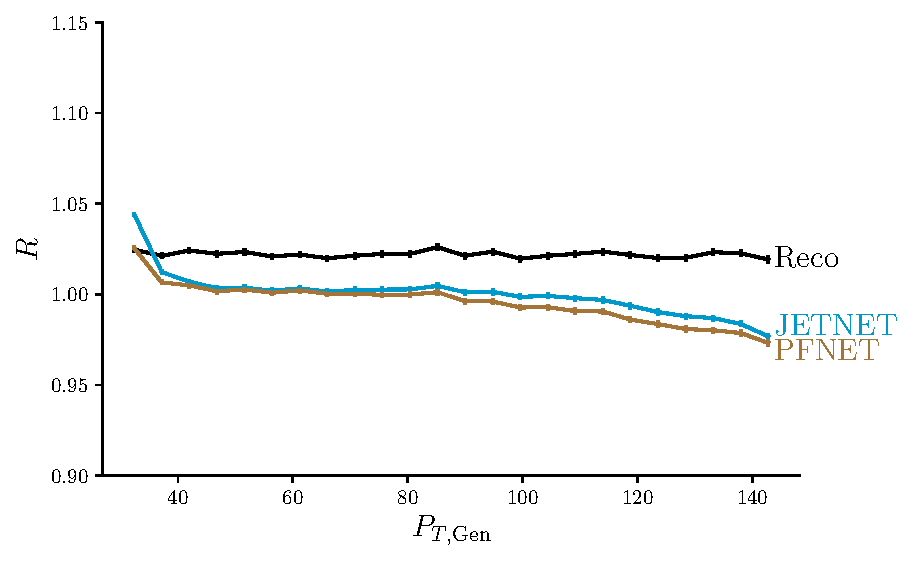
\includegraphics[width=.9\linewidth]{../images/comp_R.pdf}
  \caption{The mean values of the R distribution are represented in
    dependence to \(P_{T, \text{Gen}}\). The two networks after the
    second iteration and the Reco results are shown.}
  \label{comp_R}
\end{figure}

\begin{figure}[H]
  \centering
  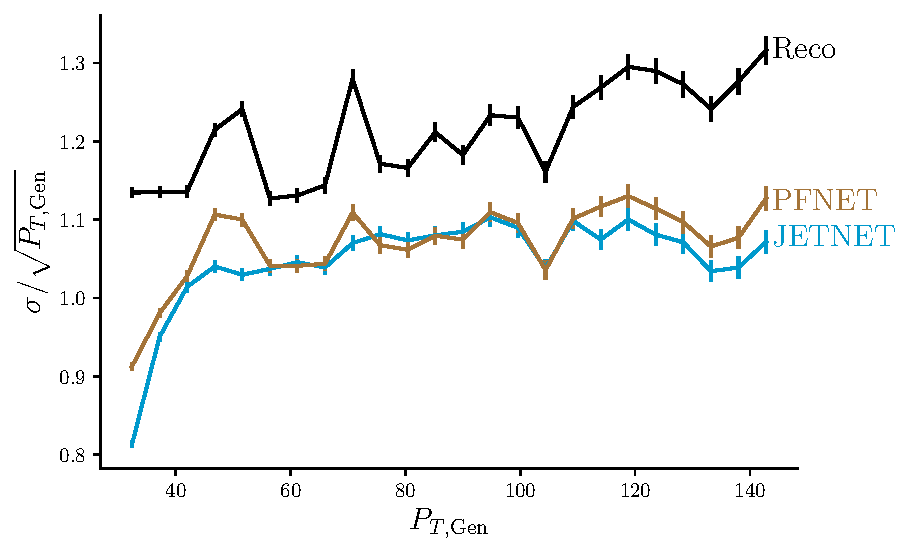
\includegraphics[width=.9\linewidth]{../images/comp_res.pdf}
  \caption{The standard deviation by the root of \(P_{T, \text{Gen}}\)
    in relation to \(P_{T, \text{Gen}}\) is represented.}
  \label{comp_res}
\end{figure}

Figure \ref{comp_res} shows that this also applies to the
resolution. The PFNet has fewer deviations from the edges. In the
middle, however, the lines are comparable.

Overall, the performance of both networks is on average about 15
percent better than that of the clustering algorithm.  It is therefore
possible to improve the pulse resolution of the jets with the help of
deep learning techniques.  For this analysis, neither the hyper
parameters were tuned nor the input variables changed. Therefore the
analysis can only show that the resolution can be improved, but not
how far this is possible. That the two architectures perform roughly
equally well is either an indication that the PFNet structure does not
provide a better result for pulse calibrations or that the unprocessed
input variables are not suitable for this type of network. Another
possibilty is that the overall performance maximum was nearly reached
by the analysis. Further analysis is needed to investigate this.  In
the same way, the alternative loss function could reduce the boundary
effect, but not eliminate it altogether.

\chapter{Conclusion}
\label{sec:org62a45ca}

A calorimeter was simulated during the work. This calorimeter was used
to  train  various  networks   in  energy  determination.  Using  data
augmentation the  overfitting of  the networks  could be  reduced. The
application of  Adversarial Training  to reduce systematic  errors was
unsuccessful.  From  the distribution of  the values, a  loss function
could   be   inferred,   which    greatly   reduces   the   systematic
deviations. The principle behind this design is universal. It could be
shown  that  a Convolutional  Neural  Net  is  better suited  for  the
regression of calorimeter data than  a Fully Connected Neural Net. The
performance of  the networks was  significantly higher than that  of a
linear fit.

In the second part of the analysis, networks for jet energy
calibration were trained.  The approach of loss function design could
be extended and reduced the systematic deviations caused by the
limited value range. In addition to a Fully Connected Neural Net, a
Particle Flow Network could also be trained. The overall performance
of the two architecture types was approximately identical. Both
network types performed about 15\% better than the jet algorithm.

All in all it could be shown that regression in particle physics is a
good field to apply deep learning. This allows to achieve better
performances than traditional algorithms. However, machine learning
algorithms still lack robustness against systematic
deviations. Further research is needed to overcome this
problem. Neither the architectural design, the hyper parameter tuning
nor the input variable design was really treated in the study. This
will be investigated in further studies. Stay tuned.


\appendix
\cleardoublepage
\bibliographystyle{unsrt}
\bibliography{bibliography}
\chapter*{Eidesstattliche Versicherung}
\thispagestyle{empty}
\addcontentsline{toc}{chapter}{Eidesstattliche Versicherung}

Ich versichere, dass ich die beigefügte schriftliche Masterarbeit selbstständig angefertigt und keine anderen als die angegebenen Hilfsmittel benutzt habe.
Alle Stellen, die dem Wortlaut oder dem Sinn nach anderen Werken entnommen sind,
habe ich in jedem einzelnen Fall unter genauer Angabe der Quelle deutlich als Entlehnung kenntlich gemacht. Dies gilt auch für alle Informationen, die dem Internet oder
anderer elektronischer Datensammlungen entnommen wurden. Ich erkläre ferner, dass
die von mir angefertigte Masterarbeit in gleicher oder ähnlicher Fassung noch nicht Bestandteil einer Studien- oder Prüfungsleistung im Rahmen meines
Studiums war. Die von mir eingereichte schriftliche Fassung entspricht jener auf dem
elektronischen Speichermedium.

\noindent Ich bin damit einverstanden, dass die Masterarbeit veröffentlicht wird.

\vspace{2cm} 

\noindent Hamburg, den \uline{~~~~~~~~~~~~~~~~~~~~}~~~~~Unterschrift: \uline{~~~~~~~~~~~~~~~~~~~~~~~~~~~~~~~~~~~~~~~~~~~~~~~~~~} 


\end{document}
